\chapter{The Universal Domain and Definitional Domain Package}
\label{ch:universal}

\section{Introduction}

In Chapters \ref{ch:holcf} and \ref{ch:powerdomain} we have seen how to construct a wide variety of type constructors for HOLCF, including strict sums and products, lifted cpos, continuous function spaces, and three kinds of powerdomains. Additionally, the \textsc{Domain} package described in Chapter~\ref{ch:domain} provides automation for defining \emph{recursive} cpo types, but there are gaps in its implementation: In particular, each new type is not actually \emph{defined}; rather, it is \emph{axiomatized} instead. Generating axioms for each definition leads to serious concerns about soundness.

This chapter describes the formalization of a universal domain that is suitable for modeling general recursive datatypes. The construction is purely definitional, introducing no new axioms. Defining recursive types in terms of this universal domain allows the new \textsc{Domain} package to derive strong reasoning principles, with soundness ensured by construction.

A \emph{universal domain} is a single cpo type that contains a large class of other cpos as subsets. The universal domain presented in this chapter is a universal \emph{bifinite} domain, meaning that any bifinite cpo can be represented within it. (See Chapter~\ref{ch:powerdomain} for a discussion of bifinite cpos.) More specifically, it is a \emph{deflation}-universal bifinite domain, because each bifinite cpo is represented as a deflation, and type constructors are represented as continuous functions on deflations. The deflation model of recursive datatypes is convenient to work with, because recursive datatypes can be defined with the same least fixed point machinery used for defining recursive functions.

Constructions of a universal bifinite domain exist in the domain theory literature~\cite{gunter87universal, gunter90semantic}. This chapter will show how to adapt one such construction so that it can be formalized in a theorem prover like Isabelle. The formalization uses the ideal completion process described previously in Chapter~\ref{ch:powerdomain} (\S\ref{sec:pd-ideal-completion}).

\paragraph{Contributions.} The original contributions presented in this chapter are:
\begin{itemize}

\item A new construction of a universal domain that can represent a wide variety of types, including sums, products, continuous function space, powerdomains, and recursive types built from these. Universal domain elements are defined in terms of sets of natural numbers, using ideal completion---thus the construction is suitable for simply-typed, higher-order logic theorem provers.

\item A formalization of this construction in the HOLCF library of the Isabelle theorem prover. The formalization is fully definitional; no new axioms are asserted.

\item A formalization of a type of algebraic deflations, which are used to represent types and type constructors. As a cpo, this type is also used to build representations of recursive datatypes as least fixed points.

\item An extension of the HOLCF \textsc{Domain} package to construct new types explicitly, replacing the isomorphism and reach axioms with actual theorems. The new \textsc{Domain} package is purely definitional, and no longer declares any axioms.

\item The definition of a class of \emph{predomain} types, which are an unpointed variant of bifinite domains. We show how predomains can be represented with algebraic deflations, and how support for predomains can be integrated into the new \textsc{Domain} package.

\end{itemize}

\paragraph{Overview.} The remainder of the chapter is organized as follows. We start with background material about embedding-projection pairs and the deflation model of recursive datatypes (\S\ref{sec:universal-background}); this material previews the implementation of the definitional \textsc{Domain} package and motivates the definition of a universal domain. Next is a summary of the user-visible interface to the HOLCF universal domain library (\S\ref{sec:universal-features}). The construction of the universal domain type itself, along with embedding and projection functions, is covered in the following section (\S\ref{sec:universal-construction}).

After defining the universal domain, we move on to algebraic deflations, which are used to formalize the class of representable domains (\S\ref{sec:universal-alg-defl}); and then to the actual implementation of the new definitional \textsc{Domain} package (\S\ref{sec:universal-package}). We also describe an unpointed variant of representable domains, called \emph{predomains}, and how they are supported by the \textsc{Domain} package (\S\ref{sec:universal-predomain}). The chapter concludes with a discussion of related work (\S\ref{sec:universal-conclusion}).

A significant portion of the material presented in this chapter is based on previously published work. The formalization of the universal domain was initially described in the author's 2009 paper \cite{huffman09universal}, which predated the completion of the definitional \textsc{Domain} package. Many of the ideas related to representable domains and deflation combinators originated in an earlier joint paper with Matthews and White \cite{huffman05axiomatic}.

\section{Background}
\label{sec:universal-background}

\subsection{Embedding-projection pairs and deflations}

Some cpos can be embedded within other cpos. The concept of an \emph{embedding-projection pair} (often shortened to \emph{ep-pair}) formalizes this notion. Let $A$ and $B$ be cpos, and $e : A \rightarrow B$ and $p : B \rightarrow A$ be continuous functions. Then $e$ and $p$ are an ep-pair if $p \circ e = \mathrm{Id}_A$ and $e \circ p \sqsubseteq \mathrm{Id}_B$. In this case, we write $(e, p) : A \stackrel{ep}{\to} B$. The existence of such an ep-pair means that cpo $A$ can be embedded in cpo $B$.
%
\indexdef{ep_pair}
\indexthm{e_inverse}
\indexthm{e_p_below}
\begin{isacode}
locale ep_pair =
  fixes e :: "'a \<rightarrow> 'b" and p :: "'b \<rightarrow> 'a"
  assumes e_inverse: "\<And>x. p\<cdot>(e\<cdot>x) = x"
  assumes e_p_below: "\<And>y. e\<cdot>(p\<cdot>y) \<sqsubseteq> y"
\end{isacode}
%
Ep-pairs have many useful properties: $e$ is injective, $p$ is surjective, both are strict, each function uniquely determines the other, and the range of $e$ is a sub-cpo of $B$. The composition of two ep-pairs yields another ep-pair: If $(e_1, p_1) : A \stackrel{ep}{\to} B$ and $(e_2, p_2) : B \stackrel{ep}{\to} C$, then $(e_2 \circ e_1, p_1 \circ p_2) : A \stackrel{ep}{\to} C$. Ep-pairs can also be lifted over many type constructors, including cartesian product and continuous function space (see Fig.~\ref{fig:universal-ep-pair-lemmas}).

\begin{figure}
\indexthm{ep_pair_comp}
\begin{isacode}
lemma ep_pair_comp:
  assumes "ep_pair e1 p1" and "ep_pair e2 p2"
  shows "ep_pair (e2 oo e1) (p1 oo p2)"
\end{isacode}
\unmedskip
\indexdef{prod_map}
\begin{isacode}
definition prod_map :: "('a \<rightarrow> 'b) \<rightarrow> ('c \<rightarrow> 'd) \<rightarrow> 'a \<times> 'c \<rightarrow> 'b \<times> 'd"
  where "prod_map = (\<Lambda> f g p. (f\<cdot>(fst p), g\<cdot>(snd p)))"
\end{isacode}
\unmedskip
\indexthm{ep_pair_prod_map}
\begin{isacode}
lemma ep_pair_prod_map:
  assumes "ep_pair e1 p1" and "ep_pair e2 p2"
  shows "ep_pair (prod_map\<cdot>e1\<cdot>e2) (prod_map\<cdot>p1\<cdot>p2)"
\end{isacode}
\unmedskip
\indexdef{cfun_map}
\begin{isacode}
definition cfun_map :: "('b \<rightarrow> 'a) \<rightarrow> ('c \<rightarrow> 'd) \<rightarrow> ('a \<rightarrow> 'c) \<rightarrow> ('b \<rightarrow> 'd)"
  where "cfun_map = (\<Lambda> a b f x. b\<cdot>(f\<cdot>(a\<cdot>x)))"
\end{isacode}
\unmedskip
\indexthm{ep_pair_cfun_map}
\begin{isacode}
lemma ep_pair_cfun_map:
  assumes "ep_pair e1 p1" and "ep_pair e2 p2"
  shows "ep_pair (cfun_map\<cdot>p1\<cdot>e2) (cfun_map\<cdot>e1\<cdot>p2)"
\end{isacode}
\caption{Lemmas for composing ep-pairs}
\label{fig:universal-ep-pair-lemmas}
\end{figure}

A continuous function $d : A \to A$ is a \emph{deflation} if it is idempotent and below the identity function: $d \circ d = d \sqsubseteq \mathrm{Id}_A$.
\pagebreak

\indexdef{deflation}
\indexthm{idem}
\indexthm{below}
\begin{isacode}
locale deflation =
  fixes d :: "'a \<rightarrow> 'a"
  assumes idem: "\<And>x. d\<cdot>(d\<cdot>x) = d\<cdot>x"
  assumes below: "\<And>x. d\<cdot>x \<sqsubseteq> x"
\end{isacode}
%
Deflations and ep-pairs are closely related. Given an ep-pair $(e, p) : A \stackrel{ep}{\to} B$, the composition $e \circ p$ is a deflation on $B$ whose image set is isomorphic to $A$. Conversely, every deflation $d : B \rightarrow B$ also gives rise to an ep-pair. Define the cpo $A$ to be the image set of $d$; also define $e$ to be the inclusion map from $A$ to $B$, and define $p = d$. Then $(e, p)$ is an embedding-projection pair. So saying that there exists an ep-pair from $A$ to $B$ is equivalent to saying that there exists a deflation on $B$ whose image set is isomorphic to $A$. Figure~\ref{fig:universal-ep-pairs} shows the relationship between ep-pairs and deflations.

\begin{figure}
\centering
\subfloat[ep-pair]{
\begin{tikzpicture}
[>=stealth, point/.style={coordinate, circle, fill, inner sep=0, outer sep=0.4mm, minimum size=1.2mm}]
\draw [xshift=-3cm] (0,0) -- (-2.5, 2.5) -- (-0.5, 2.5) -- cycle;
\draw (0, 0) -- (-4, 4) -- (1.5, 4) -- cycle;
\draw [dashed] (0, 0) -- (-0.5, 2.5) -- (-2.5, 2.5);
\node (1a) [point] at (-0.6, 1.1);
\node (1b) [point, xshift=-3cm] at (-0.6, 1.1);
\node (2a) [point] at (-1.5, 2.5);
\node (2b) [point, xshift=-3cm] at (-1.5, 2.5);
\node (3a) [point] at (-1.6, 3.7);
\path (1a) edge [->, bend right=20, above] node {\small $p$} (1b);
\path (1b) edge [->, bend right=20, below] node {\small $e$} (1a);
\path (2a) edge [->, bend right=20, above, pos=0.65] node {\small $p$} (2b);
\path (2b) edge [->, bend right=20, below] node {\small $e$} (2a);
\path (3a) edge [->, bend right=35, above, near end] node {\small $p$} (2b);
\path (3a) edge [dotted, right] node {\small $\sqsubseteq$} (2a);
\end{tikzpicture}
}
\hfill
\subfloat[deflation]{
\begin{tikzpicture}
[>=stealth, point/.style={coordinate, circle, fill, inner sep=0, outer sep=0.4mm, minimum size=1.2mm}]
\draw (0, 0) -- (-4, 4) -- (1.5, 4) -- cycle;
\draw [dashed] (0, 0) -- (-0.5, 2.5) -- (-2.5, 2.5);
\node (1a) [point] at (-0.6, 1.2);
\node (2a) [point] at (-1.5, 2.5);
\node (3a) [point] at (-1.6, 3.7);
\path (1a) edge [->, loop below, right] node {\small $d$} (1a);
\path (2a) edge [->, loop below, right] node {\small $d$} (2a);
\path (3a) edge [->, right] node {\small $d$} (2a);
\end{tikzpicture}
}
\caption{Embedding-projection pairs and deflations}
\label{fig:universal-ep-pairs}
\end{figure}

A deflation is a function, but it can also be viewed as a set: Just take the image of the function, or equivalently, its set of fixed points---for idempotent functions they are the same. The dashed outline in Fig.~\ref{fig:universal-ep-pairs} shows the set defined by the deflation $d$. Every deflation on a cpo $A$ gives a set that is a sub-cpo, and contains $\bot$ if $A$ has a least element. Not all sub-cpos have a corresponding deflation, but if one exists then it is unique. The set-oriented and function-oriented views of deflations also give the same ordering: For any deflations $f$ and $g$, $f \sqsubseteq g$ if and only if $\mathrm{Im}(f) \subseteq \mathrm{Im}(g)$.

\subsection{Deflation model of datatypes}
\label{sec:universal-deflation}

We say that a type $A$ is \emph{representable} in $U$ if there exists an ep-pair from $A$ to $U$, or equivalently if there exists a deflation $d_A$ on $U$ whose image $\mathrm{Im}(d)$ is isomorphic to $A$. We say that $U$ is a \emph{universal domain} for some class of cpos if every cpo in the class is representable in $U$.

While types can be represented by deflations, type \emph{constructors} (which are like functions from types to types) can be represented as functions from deflations to deflations. We say that a type constructor $F$ is representable in $U$ if there exists a continuous function $\Phi$, mapping from deflations to deflations, such that $\mathrm{Im}(\Phi(d))$ is isomorphic to $F(\mathrm{Im}(d))$. Such deflation combinators can be used to build deflations for recursive datatypes \cite[\S7]{gunter90semantic}. The remainder of this section will show how this process works, by example. The new definitional \textsc{Domain} package uses the same process to construct recursive datatypes, as will be explained in Sec.~\ref{sec:universal-package}.

To illustrate the concepts of ep-pairs, deflations, and representable types, we will examine some concrete implementations of these ideas in Haskell. We start by defining a universal Haskell datatype \hs{U}, which should be able to encode every datatype definable in Haskell.
%
\begin{hscode}
data U = Con String [U] | Fun (U -> U)
\end{hscode}
%
Type \hs{U} has two constructors, \hs{Con} and \hs{Fun}. For encoding ordinary algebraic datatypes like pairs, lists, or trees, we only need to use \hs{Con}. The string identifies the constructor name; the list contains each of its encoded arguments. The constructor \hs{Fun} is required for the function space type \hs{(->)} and other datatypes containing functions.

We then define a Haskell type class \hs{Rep} for ``representable'' Haskell types. We expect that for each \hs{Rep} class instance, \hs{emb} and \hs{prj} should always form an ep-pair.
%
\begin{hscode}
class Rep a where
  emb :: a -> U
  prj :: U -> a
\end{hscode}

\paragraph{Booleans are representable.} Below we make the standard Haskell type \hs{Bool} an instance of class \hs{Rep}. To check that \hs{emb} and \hs{prj} are an ep-pair, we can see that \hs{prj} is the inverse of \hs{emb}. Also, we can see that \hs{prj} is as ``undefined'' as possible---it maps every ill-formed value to $\bot$. Given the definition of \hs{emb}, this is the only definition of \hs{prj} that will yield an ep-pair.
%
\begin{hscode}
instance Rep Bool where
  emb True             = Con "True" []
  emb False            = Con "False" []
  prj (Con "True" [])  = True
  prj (Con "False" []) = False
  prj _                = undefined
\end{hscode}
%
The Haskell type \hs{Bool} is represented by the function \hs{tBool}, a deflation which is equal to the composition \hs{(emb . prj)} for type \hs{Bool}. For an input that corresponds to a well-formed encoded boolean, \hs{tBool} maps the input to itself. Any other input is mapped to $\bot$.
%
\begin{hscode}
tBool :: U -> U
tBool (Con "True" [])  = Con "True" []
tBool (Con "False" []) = Con "False" []
tBool _                = undefined
\end{hscode}

\paragraph{Lists are representable.} Next we will consider the standard Haskell list data\-type. We will create an ep-pair from type \hs{[a]} to \hs{U} as a composition of two ep-pairs, with \hs{[U]} used as an intermediate type. The functions \hs{embList} and \hs{prjList} form an ep-pair from \hs{[U]} to \hs{U}.
%
\begin{hscode}
embList :: [U] -> U
embList []       = Con "[]" []
embList (x : xs) = Con ":" [x, embList xs]

prjList :: U -> [U]
prjList (Con "[]" [])     = []
prjList (Con ":" [x, xs]) = x : prjList xs
prjList _                 = undefined
\end{hscode}
%
To build an ep-pair from \hs{[a]} to \hs{[U]}, we can use the \hs{emb} and \hs{prj} functions for the element type \hs{a}, noting that the standard \hs{map} function for lists preserves ep-pairs. Finally, we can define \hs{emb} and \hs{prj} on lists using function composition:
%
\begin{hscode}
instance Rep a => Rep [a] where
  emb = embList . map emb
  prj = map prj . prjList
\end{hscode}
%
The list type constructor can be represented by the function \hs{tList}, shown below. 
%
\begin{hscode}
tList :: (U -> U) -> (U -> U)
tList d = embList . map d . prjList
\end{hscode}
%
We can see that if \hs{d} is a deflation, then so is \hs{tList d}. It is also easy to verify that \hs{tList} actually does represent the list type constructor: If \hs{d} is equal to \hs{(emb . prj)} for type \hs{a},  then \hs{tList d} is equal to \hs{(emb . prj)} for type \hs{[a]}.

Testing these functions on some example inputs can give us a better idea of how they work. As expected, the deflation \hs{tList tBool} maps any value that corresponds to an encoded list of booleans to itself. For example, \hs{tList tBool} leaves the result of \hs{emb [True, False]} unchanged:
%
\begin{hscode}
emb [True, False] =
  Con ":" [Con "True" [], Con ":" [Con "False" [], Con "[]" []]]
\end{hscode}
\unmedskip
\begin{hscode}
tList tBool
 (Con ":" [Con "True" [], Con ":" [Con "False" [], Con "[]" []]])
 = Con ":" [Con "True" [], Con ":" [Con "False" [], Con "[]" []]]
\end{hscode}
%
When applied to an ill-formed argument, however, a deflation like \hs{tList tBool} has the effect of replacing any ill-formed portions of the input with \hs{undefined}:
\begin{hscode}
tList tBool
  (Con ":" [Con "bogus" [],
            Con ":" [Con "False" [], Con "wrong" []]])
  = Con ":" [undefined, Con ":" [Con "False" [], undefined]]
\end{hscode}

\paragraph{Representability of function space.} The approach used for lists can be generalized to any other type constructor with a map function---even contravariant types like the function space. We start by defining functions \hs{embFun} and \hs{prjFun}, which form an ep-pair between types \hs{U -> U} and \hs{U}.
%
\begin{hscode}
embFun :: (U -> U) -> U
embFun !f = Fun f

prjFun :: U -> (U -> U)
prjFun (Fun f) = f
prjFun _ = undefined
\end{hscode}
%
The strictness annotation (\hs{!f}) is necessary to make \hs{embFun} strict, because Haskell functions with variable patterns are lazy by default. (Both components of an ep-pair must be strict functions.)

Next, we define a \hs{map}-like operator for the Haskell function type \hs{(->)}. The type of the argument \hs{a :: a2 -> a1} reflects the fact that the function space type constructor is contravariant in its left argument.
%
\begin{hscode}
mapFun :: (a2 -> a1) -> (b1 -> b2) -> (a1 -> b1) -> (a2 -> b2)
mapFun a b !f = b . f . a
\end{hscode}
%
Finally, we can define a class instance for the function type \hs{a -> b}.
%
\begin{hscode}
instance (Rep a, Rep b) => Rep (a -> b) where
  emb = embFun . mapFun prj emb
  prj = mapFun emb prj . prjFun
\end{hscode}
%
For the list example, \hs{emb} on lists only calls \hs{emb} on the element type, and similarly \hs{prj} calls only \hs{prj}. But because the function type \hs{a -> b} is contravariant in \hs{a}, we have \hs{emb :: (a -> b) -> U} calling \hs{prj :: U -> a}, and \hs{prj :: U -> (a -> b)} calling \hs{emb :: a -> U}.

The function \hs{tFun} represents the Haskell function space type constructor \hs{(->)}. If \hs{a} and \hs{b} are both deflations, then \hs{tFun a b} will be a deflation also.
%
\begin{hscode}
tFun :: (U -> U) -> (U -> U) -> (U -> U)
tFun a b = embFun . mapFun a b . prjFun
\end{hscode}
%
\paragraph{Recursive definitions of deflations.} Using the deflation combinators \hs{tBool}, \hs{tList}, and \hs{tFun}, we can recursively define new deflations that represent recursive datatypes. For example, consider the deflations \hs{tD} and \hs{tE} below:
%
\begin{hscode}
tD, tE :: U -> U
tD = tFun tBool (tList tD)
tE = tFun (tList tE) tE
\end{hscode}
%
The image set of \hs{tD} is a cpo \hs{D} that satisfies the equation \hs{D} = \hs{Bool -> [D]}. Likewise, the image set of \hs{tE} is a cpo \hs{E} that satisfies \hs{E} = \hs{[E] -> E}. In general, we can recursively define a deflation for any given type equation of the form $T = F(T)$, where $F(T)$ is a type expression involving type constructors (like \hs{Bool}, \hs{[]}, or \hs{(->)}) for which we have deflation combinators.

Thus by using the deflation model, we can solve type equations with ordinary recursive value definitions. This is a significant benefit for HOLCF, because it means that the theory of least fixed points used by the \textsc{Fixrec} package can all be reused in the new definitional \textsc{Domain} package. As a prerequisite for solving type equations, the \textsc{Domain} package needs deflation combinators for all the basic HOLCF types. And as we have seen above, defining the deflation combinators will require ep-pairs from each basic HOLCF type into the universal domain.

\section{Universal domain library features}
\label{sec:universal-features}

The universal domain library is large (about 1000 lines of definitions and proof scripts), defining various types and numerous functions and constants. However, most of these are for internal use only. Just a few parts of the library are directly relevant for users: There is the universal domain type \isa{udom}, which is an instance of the \isa{bifinite} class, along with the following three functions:
%
\indexdef{udom_emb}
\indexdef{udom_prj}
\indexdef{udom_approx}
\begin{isacode}
udom_emb :: "(nat => 'a -> 'a) => 'a -> udom"
udom_prj :: "(nat => 'a -> 'a) => udom -> 'a"
udom_approx :: "nat => udom -> udom"
\end{isacode}
%
The functions \isa{udom_emb} and \isa{udom_prj} give an ep-pair from type \isa{'a} to \isa{udom}. They are parameterized by a chain of approx functions on type \isa{'a}.
%
\indexthm{ep_pair_udom}
\begin{isacode}
lemma ep_pair_udom:
  assumes "approx_chain a"
  shows "ep_pair (udom_emb a) (udom_prj a)"
\end{isacode}
%
Recall the definition of approx-chains, used in the previous chapter for defining the class of bifinite cpos. A cpo is bifinite if an approx-chain exists for that type.
%
\indexdef{approx_chain}
\indexthm{chain_approx}
\indexthm{lub_approx}
\indexthm{finite_deflation_approx}
\begin{isacode}
locale approx_chain =
  fixes approx :: "nat \<Rightarrow> 'a \<rightarrow> 'a"
  assumes chain_approx: "chain (\<lambda>i. approx i)"
  assumes lub_approx: "(\<Squnion>i. approx i) = ID"
  assumes finite_deflation_approx: "\<And>i. finite_deflation (approx i)"
\end{isacode}
%
In order to help build approx-chains for other types, the universal domain library provides \isa{udom_approx}, which is an approx-chain for type \isa{udom}.
%
\indexthm{udom_approx}
\begin{isacode}
lemma udom_approx: "approx_chain udom_approx"
\end{isacode}
%
We can use all three \isa{udom} functions in combination to yield ep-pairs for types like \isa{udom \<times> udom}. Using \isa{udom_approx} with the map combinator \isa{prod_map}, which preserves finite deflations, yields an approx-chain on type \isa{udom \<times> udom}. Then the \isa{udom_emb} and \isa{udom_prj} functions give the desired ep-pair.
%
\indexdef{prod_emb}
\begin{isacode}
definition prod_emb :: "udom \<times> udom \<rightarrow> udom"
  where "prod_emb =
    udom_emb (\<lambda>i. prod_map\<cdot>(udom_approx i)\<cdot>(udom_approx i))"
\end{isacode}
\unmedskip
\indexdef{prod_prj}
\begin{isacode}
definition prod_prj :: "udom \<rightarrow> udom \<times> udom"
  where "prod_prj = udom_prj (\<lambda>i. prod_map\<cdot>(udom_approx i)\<cdot>(udom_approx i))"
\end{isacode}
\unmedskip
\begin{isacode}
lemma ep_pair_prod: "ep_pair prod_emb prod_prj"
\end{isacode}
%
Embedding-projection pairs are defined similarly for all of the other type constructors defined in HOLCF: $\to$, $\otimes$, $\oplus$, $-_\bot$, $(-)^\sharp$, $(-)^\flat$, and $(-)^\natural$. These ep-pairs are used to define deflation combinators that represent each type constructor; in turn, these combinators are used to construct solutions to recursive domain equations. Details of this process will be covered fully in Sections \ref{sec:universal-alg-defl} and \ref{sec:universal-package}.

\section{Construction of the universal domain}
\label{sec:universal-construction}

Informally, a \emph{bifinite domain} is a cpo that can be written as the limit of a sequence of finite partial orders. This section describes how to construct a \emph{universal} bifinite domain $\mathcal{U}$, along with an ep-pair from another arbitrary bifinite domain $D$ into $\mathcal{U}$. The general strategy is as follows:
\begin{itemize}
\item From the bifinite structure of $D$, obtain a sequence of finite posets $P_n$ whose limit is $D$.
\item Following Gunter \cite{gunter87universal}, decompose the sequence $P_n$ further into a sequence of \emph{increments} that insert new elements one at a time.
\item Construct a universal domain basis that can encode any increment.
\item Construct the actual universal domain $\mathcal{U}$ using ideal completion.
\item Define the embedding and projection functions between $D$ and $\mathcal{U}$ using continuous extension, in terms of their action on basis elements.
\end{itemize}

The process of constructing a sequence of increments is described in Sec.~\ref{sec:universal-increments}. The underlying theory is standard, so the section is primarily exposition; the original contribution here is the formalization of that work in a theorem prover. The remainder of the construction, including the basis and embedding/projection functions, is covered in Sec.~\ref{sec:universal-basis} onwards; here both the theory and the formalization are original.

\subsection{Building a sequence of increments}
\label{sec:universal-increments}

Any bifinite domain $D$ can be represented as the limit of a sequence of finite posets, with embedding-projection pairs between each successive pair. Figure~\ref{fig:posets} shows the first few posets from one such sequence.

\begin{figure}
\begin{center}
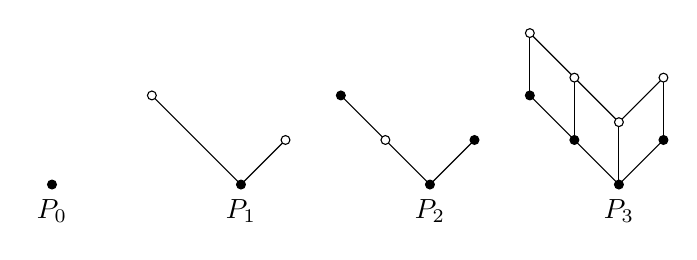
\begin{tikzpicture}[scale=0.8]
  \begin{scope}[rotate=45]
    \filldraw (0,0) circle (2pt);
    \draw (-0.3, -0.3) node {$P_0$};
  \end{scope}
  \begin{scope}[xshift=3cm,rotate=45]
    \draw (0.0, 0.0) -- (0.0, 2.0);
    \draw (0.0, 0.0) -- (1.0, 0.0);
    \filldraw[fill=black] (0.0, 0.0) circle (2pt);
    \filldraw[fill=white] (0.0, 2.0) circle (2pt);
    \filldraw[fill=white] (1.0, 0.0) circle (2pt);
    \draw (-0.3, -0.3) node {$P_1$};
  \end{scope}
  \begin{scope}[xshift=6cm,rotate=45]
    \draw (0.0, 0.0) -- (0.0, 2.0);
    \draw (0.0, 0.0) -- (1.0, 0.0);
    \filldraw[fill=black] (0.0, 0.0) circle (2pt);
    \filldraw[fill=black] (0.0, 2.0) circle (2pt);
    \filldraw[fill=black] (1.0, 0.0) circle (2pt);
    \filldraw[fill=white] (0.0, 1.0) circle (2pt);
    \draw (-0.3, -0.3) node {$P_2$};
  \end{scope}
  \begin{scope}[xshift=9cm,rotate=45]
    \draw (0.0, 2.0) -- (0.0, 0.0) -- (1.0, 0.0);
    \draw (0.7, 2.7) -- (0.7, 0.7) -- (1.7, 0.7);
    \draw (0.0, 2.0) -- (0.7, 2.7);
    \draw (0.0, 1.0) -- (0.7, 1.7);
    \draw (0.0, 0.0) -- (0.7, 0.7);
    \draw (1.0, 0.0) -- (1.7, 0.7);
    \filldraw[fill=black] (0.0, 0.0) circle (2pt);
    \filldraw[fill=black] (0.0, 2.0) circle (2pt);
    \filldraw[fill=black] (0.0, 1.0) circle (2pt);
    \filldraw[fill=black] (1.0, 0.0) circle (2pt);
    \filldraw[fill=white] (0.7, 0.7) circle (2pt);
    \filldraw[fill=white] (0.7, 2.7) circle (2pt);
    \filldraw[fill=white] (0.7, 1.7) circle (2pt);
    \filldraw[fill=white] (1.7, 0.7) circle (2pt);
    \draw (-0.3, -0.3) node {$P_3$};
  \end{scope}
\end{tikzpicture}
\end{center}
\caption{A sequence of finite posets. Each $P_n$ can be embedded into $P_{n+1}$; black nodes indicate the range of the embedding function.}
\label{fig:posets}
\end{figure}

In each step along the chain, each new poset $P_{n+1}$ is larger than the previous $P_n$ by some finite amount; the structure of $P_{n+1}$ has $P_n$ embedded within it, but it has some new elements as well.

An ep-pair between finite posets $P$ and $P'$, where $P'$ has exactly one more element than $P$, is called an \emph{increment} (terminology due to Gunter \cite{gunter92semantics}). In Fig.~\ref{fig:posets}, the embedding of $P_1$ into $P_2$ is an example of an increment.

The strategy for embedding a bifinite domain into the universal domain is built around increments. The universal domain is designed so that if a finite partial order $P$ is representable (i.e., by a deflation), and there is an increment from $P$ to $P'$, then $P'$ will also be representable.

For all embeddings from $P_n$ to $P_{n+1}$ that add more than one new value, we will need to decompose the single large embedding into a sequence of smaller increments. The challenge, then, is to determine in which order the new elements should be inserted. The order matters: Adding elements in the wrong order can cause problems, as shown in Fig.~\ref{fig:order}.

\begin{figure}
\begin{center}
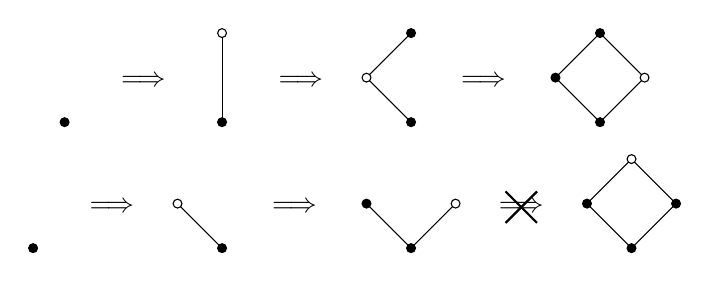
\begin{tikzpicture}[scale=0.8]
  \begin{scope}[xshift=0cm,rotate=45]
    \filldraw (0,0) circle (2pt);
  \end{scope}
  \begin{scope}[xshift=3.0cm,rotate=45]
    \draw (0.0, 0.0) -- (0.0, 1.0);
    \filldraw[fill=black] (0.0, 0.0) circle (2pt);
    \filldraw[fill=white] (0.0, 1.0) circle (2pt);
  \end{scope}
  \begin{scope}[xshift=6.0cm,rotate=45]
    \draw (0.0, 0.0) -- (0.0, 1.0);
    \draw (0.0, 0.0) -- (1.0, 0.0);
    \filldraw[fill=black] (0.0, 0.0) circle (2pt);
    \filldraw[fill=black] (0.0, 1.0) circle (2pt);
    \filldraw[fill=white] (1.0, 0.0) circle (2pt);
  \end{scope}
  \begin{scope}[xshift=9.5cm,rotate=45]
    \draw (0.0, 1.0) -- (0.0, 0.0) -- (1.0, 0.0);
    \draw (0.0, 1.0) -- (1.0, 1.0) -- (1.0, 0.0);
    \filldraw[fill=black] (0.0, 0.0) circle (2pt);
    \filldraw[fill=black] (0.0, 1.0) circle (2pt);
    \filldraw[fill=black] (1.0, 0.0) circle (2pt);
    \filldraw[fill=white] (1.0, 1.0) circle (2pt);
  \end{scope}
  \draw (1.25, 0.65) node {$\Longrightarrow$};
  \draw (4.15, 0.65) node {$\Longrightarrow$};
  \draw (7.75, 0.65) node {$\Longrightarrow$};
  \draw[thick] (7.5, 0.4) -- (8.0, 0.9);
  \draw[thick] (7.5, 0.9) -- (8.0, 0.4);

  \begin{scope}[xshift=0.5cm,yshift=2cm]
  \begin{scope}[xshift=0cm,rotate=45]
    \filldraw (0,0) circle (2pt);
  \end{scope}
  \begin{scope}[xshift=2.5cm,rotate=45]
    \draw (0.0, 0.0) -- (1.0, 1.0);
    \filldraw[fill=black] (0.0, 0.0) circle (2pt);
    \filldraw[fill=white] (1.0, 1.0) circle (2pt);
  \end{scope}
  \begin{scope}[xshift=5.5cm,rotate=45]
    \draw (0.0, 0.0) -- (0.0, 1.0) -- (1.0, 1.0);
    \filldraw[fill=black] (0.0, 0.0) circle (2pt);
    \filldraw[fill=black] (1.0, 1.0) circle (2pt);
    \filldraw[fill=white] (0.0, 1.0) circle (2pt);
  \end{scope}
  \begin{scope}[xshift=8.5cm,rotate=45]
    \draw (0.0, 0.0) -- (0.0, 1.0) -- (1.0, 1.0);
    \draw (0.0, 0.0) -- (1.0, 0.0) -- (1.0, 1.0);
    \filldraw[fill=black] (0.0, 0.0) circle (2pt);
    \filldraw[fill=black] (1.0, 1.0) circle (2pt);
    \filldraw[fill=black] (0.0, 1.0) circle (2pt);
    \filldraw[fill=white] (1.0, 0.0) circle (2pt);
  \end{scope}
  \draw (1.25, 0.65) node {$\Longrightarrow$};
  \draw (3.75, 0.65) node {$\Longrightarrow$};
  \draw (6.65, 0.65) node {$\Longrightarrow$};
  \end{scope}
\end{tikzpicture}
\end{center}
\caption{The right (top) and wrong (bottom) way to order insertions. No ep-pair exists between the 3-element and 4-element posets on the bottom row.}
\label{fig:order}
\end{figure}

To describe the position of a newly-inserted element, it will be helpful to invent some terminology. The set of elements \emph{above} the new element will be known as its \emph{superiors}. An element immediately \emph{below} the new element will be known as its \emph{subordinate}. (These terms are not in standard usage.)

In order for the insertion of a new element to be a valid increment, it must have exactly one subordinate. The subordinate indicates the value that the increment's projection maps the new value onto.

With the four-element poset in Fig.~\ref{fig:order}, it is not possible to insert the top element last. The reason is that the element has two subordinates: If a projection function maps the new element to one, the ordering relation with the other will not be preserved. Thus a monotone projection does not exist.

A strategy for successfully avoiding such situations is to always insert maximal elements first \cite[\S5]{gunter87universal}. Fig.~\ref{fig:increments} shows this strategy in action. Notice that the number of superiors varies from step to step, but each inserted element always has exactly one subordinate. To maintain this invariant, the least of the four new values must be inserted last.

\begin{figure}
\begin{center}
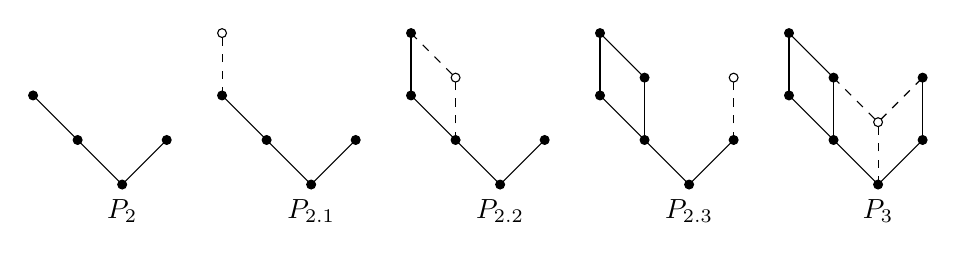
\begin{tikzpicture}[scale=0.8]
  \begin{scope}[xshift=0cm,rotate=45]
    \draw (0.0, 2.0) -- (0.0, 0.0) -- (1.0, 0.0);
    \filldraw[fill=black] (0.0, 0.0) circle (2pt);
    \filldraw[fill=black] (0.0, 2.0) circle (2pt);
    \filldraw[fill=black] (0.0, 1.0) circle (2pt);
    \filldraw[fill=black] (1.0, 0.0) circle (2pt);
    \draw (-0.3, -0.3) node {$P_2$};
  \end{scope}
  \begin{scope}[xshift=3cm,rotate=45]
    \draw (0.0, 2.0) -- (0.0, 0.0) -- (1.0, 0.0);
    \draw[dashed] (0.0, 2.0) -- (0.7, 2.7);
    \filldraw[fill=black] (0.0, 0.0) circle (2pt);
    \filldraw[fill=black] (0.0, 2.0) circle (2pt);
    \filldraw[fill=black] (0.0, 1.0) circle (2pt);
    \filldraw[fill=black] (1.0, 0.0) circle (2pt);
    \filldraw[fill=white] (0.7, 2.7) circle (2pt);
    \draw (-0.3, -0.3) node {$P_{2.1}$};
  \end{scope}
  \begin{scope}[xshift=6cm,rotate=45]
    \draw (0.0, 2.0) -- (0.0, 0.0) -- (1.0, 0.0);
    \draw (0.0, 2.0) -- (0.7, 2.7);
    \draw[dashed] (0.7, 2.7) -- (0.7, 1.7);
    \draw[dashed] (0.0, 1.0) -- (0.7, 1.7);
    \filldraw[fill=black] (0.0, 0.0) circle (2pt);
    \filldraw[fill=black] (0.0, 2.0) circle (2pt);
    \filldraw[fill=black] (0.0, 1.0) circle (2pt);
    \filldraw[fill=black] (1.0, 0.0) circle (2pt);
    \filldraw[fill=black] (0.7, 2.7) circle (2pt);
    \filldraw[fill=white] (0.7, 1.7) circle (2pt);
    \draw (-0.3, -0.3) node {$P_{2.2}$};
  \end{scope}
  \begin{scope}[xshift=9cm,rotate=45]
    \draw (0.0, 2.0) -- (0.0, 0.0) -- (1.0, 0.0);
    \draw (0.0, 2.0) -- (0.7, 2.7);
    \draw (0.7, 2.7) -- (0.7, 1.7);
    \draw (0.0, 1.0) -- (0.7, 1.7);
    \draw[dashed] (1.0, 0.0) -- (1.7, 0.7);
    \filldraw[fill=black] (0.0, 0.0) circle (2pt);
    \filldraw[fill=black] (0.0, 2.0) circle (2pt);
    \filldraw[fill=black] (0.0, 1.0) circle (2pt);
    \filldraw[fill=black] (1.0, 0.0) circle (2pt);
    \filldraw[fill=black] (0.7, 2.7) circle (2pt);
    \filldraw[fill=black] (0.7, 1.7) circle (2pt);
    \filldraw[fill=white] (1.7, 0.7) circle (2pt);
    \draw (-0.3, -0.3) node {$P_{2.3}$};
  \end{scope}
  \begin{scope}[xshift=12cm,rotate=45]
    \draw (0.0, 2.0) -- (0.0, 0.0) -- (1.0, 0.0);
    \draw (0.0, 2.0) -- (0.7, 2.7);
    \draw (0.7, 2.7) -- (0.7, 1.7);
    \draw (0.0, 1.0) -- (0.7, 1.7);
    \draw (1.0, 0.0) -- (1.7, 0.7);
    \draw[dashed] (0.7, 1.7) -- (0.7, 0.7) -- (1.7, 0.7);
    \draw[dashed] (0.0, 0.0) -- (0.7, 0.7);
    \filldraw[fill=black] (0.0, 0.0) circle (2pt);
    \filldraw[fill=black] (0.0, 2.0) circle (2pt);
    \filldraw[fill=black] (0.0, 1.0) circle (2pt);
    \filldraw[fill=black] (1.0, 0.0) circle (2pt);
    \filldraw[fill=black] (0.7, 2.7) circle (2pt);
    \filldraw[fill=black] (0.7, 1.7) circle (2pt);
    \filldraw[fill=black] (1.7, 0.7) circle (2pt);
    \filldraw[fill=white] (0.7, 0.7) circle (2pt);
    \draw (-0.3, -0.3) node {$P_3$};
  \end{scope}
\end{tikzpicture}
\end{center}
\caption{A sequence of four increments going from $P_2$ to $P_3$. Each new node may have any number of upward edges, but only one downward edge.}
\label{fig:increments}
\end{figure}

Armed with this strategy, we can finally formalize the complete sequence of increments for type $D$. To each element $x$ of the basis of $D$ we must assign a sequence number $\mathit{place}(x)$---this numbering tells in which order to insert the values. The HOLCF formalization breaks up the definition of \emph{place} as follows. First, each basis value is assigned to a rank, where $\mathit{rank}(x) = n$ means that the basis value $x$ first appears in the poset $P_n$. Equivalently, $\mathit{rank}(x)$ is the least $n$ such that $\mathit{approx}_n(x) = x$, where $\mathit{approx}_n$ is the finite deflation on $D$ with image $P_n$. Then an auxiliary function $\mathit{pos}$ assigns sequence numbers to values in finite sets, by repeatedly removing an arbitrary maximal element until the set is empty. Finally, $\mathit{place}(x)$ is defined as the sequence number of $x$ within its (finite) rank set, plus the total cardinality of all earlier ranks.
%
\begin{align}
\mathit{choose}(A) & = (\varepsilon x \in A.\ \forall y \in A.\ x \sqsubseteq y \longrightarrow x = y)
\\
pos(A,x) & =
\begin{cases} 
  0,  & \mbox{if }x = \mathit{choose}(A) \\
  1 + \mathit{pos}(A - \{\mathit{choose}(A)\}, x), & \mbox{if }x \neq \mathit{choose}(A)
\end{cases}
\\
\mathit{place}(x) & = \mathit{pos}(\{y \mid \mathit{rank}(y) = \mathit{rank}(x)\}, x) + \lVert\{y \mid \mathit{rank}(x) < \mathit{rank}(y)\}\rVert
\end{align}
For the remainder of this chapter, it will be sufficient to note that the \emph{place} function satisfies the following two properties:
%
\begin{theorem} Values in earlier ranks come before values in later ranks: If $\mathit{rank}(x) < \mathit{rank}(y)$, then $\mathit{place}(x) < \mathit{place}(y)$.
\end{theorem}
\begin{theorem} Within the same rank, larger values come first: If $\mathit{rank}(x) = \mathit{rank}(y)$ and $x \sqsubseteq y$, then $\mathit{place}(y) < \mathit{place}(x)$.
\end{theorem}

\subsection{A basis for the universal domain}
\label{sec:universal-basis}

Constructing a partial order incrementally, there are two possibilities for any newly inserted value:
%
\begin{itemize}
\item The value is the very first one (i.e., it is $\bot$)
\item The value is inserted above some previous value (its subordinate), and below zero or more other previous values (its superiors)
\end{itemize}
%
Accordingly, we can define a recursive datatype $B$ to describe the position of these values relative to each other.
%
\begin{equation}
B \mathrel{\mathop:}= \bot \mid \langle i, a, S\rangle, \mbox{where $i \in \mathbb{N}$, $a \in B$, and $S \in \mathcal{P}_f(B)$}
\end{equation}
%
The notation $\langle i, a, S\rangle$ indicates the value with serial number $i$, subordinate $a$, and the finite set of superiors $S$. (The serial number allows us to distinguish between subsequent values inserted in similar positions.)

The above definition of $B$ does not work as a datatype definition in Isabelle{\slash}HOL, because the finite set type constructor does not work with the datatype package. (Indirect recursion only works with other inductive datatypes.)  But it turns out that we do not need the datatype package at all---the type $B$ is actually isomorphic to the natural numbers. Using the bijections $\mathbb{N} \cong 1 + \mathbb{N}$ and $\mathbb{N} \cong \mathbb{N} \times \mathbb{N}$ with $\mathbb{N} \cong \mathcal{P}_f(\mathbb{N})$, we can construct a bijection that lets us use $\mathbb{N}$ as the basis datatype:
%
\begin{equation}
\mathbb{N} \cong
  1 + \mathbb{N} \times \mathbb{N} \times \mathcal{P}_f(\mathbb{N})
\end{equation}

\begin{figure}
\begin{singlespace}
\begin{center}
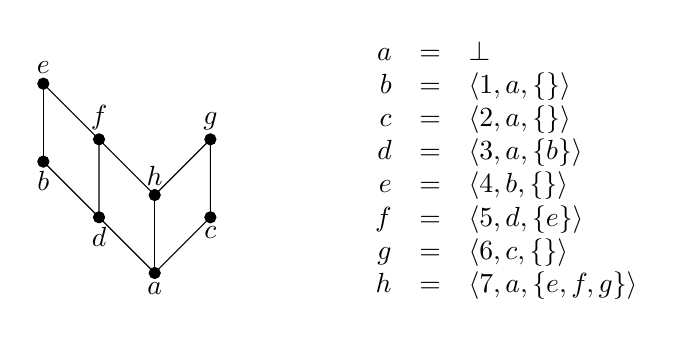
\begin{tikzpicture}
  \begin{scope}[rotate=45]
    \draw (0.0, 2.0) -- (0.0, 0.0) -- (1.0, 0.0);
    \draw (0.0, 2.0) -- (0.7, 2.7);
    \draw (0.7, 2.7) -- (0.7, 1.7);
    \draw (0.0, 1.0) -- (0.7, 1.7);
    \draw (1.0, 0.0) -- (1.7, 0.7);
    \draw (0.7, 1.7) -- (0.7, 0.7) -- (1.7, 0.7);
    \draw (0.0, 0.0) -- (0.7, 0.7);
    \filldraw (0.0, 0.0) circle (2pt) node[below] {$a$};
    \filldraw (0.0, 2.0) circle (2pt) node[below] {$b$};
    \filldraw (1.0, 0.0) circle (2pt) node[below] {$c$};
    \filldraw (0.0, 1.0) circle (2pt) node[below] {$d$};
    \filldraw (0.7, 2.7) circle (2pt) node[above] {$e$};
    \filldraw (0.7, 1.7) circle (2pt) node[above] {$f$};
    \filldraw (1.7, 0.7) circle (2pt) node[above] {$g$};
    \filldraw (0.7, 0.7) circle (2pt) node[above] {$h$};
  \end{scope}
  \draw (2.5, -0.5) node[above right] {
    $\begin{array}{rcl}
    a & = & \bot \\
    b & = & \langle 1, a, \{ \} \rangle \\
    c & = & \langle 2, a, \{ \} \rangle \\
    d & = & \langle 3, a, \{b\} \rangle \\
    e & = & \langle 4, b, \{ \} \rangle \\
    f & = & \langle 5, d, \{e\} \rangle \\
    g & = & \langle 6, c, \{ \} \rangle \\
    h & = & \langle 7, a, \{e,f,g\} \rangle
    \end{array}$
  };
\end{tikzpicture}
\end{center}
\end{singlespace}
\caption{Embedding elements of $P_3$ into the universal domain basis.}
\label{fig:encoding}
\end{figure}

Figure~\ref{fig:encoding} shows how this system works for embedding all the elements from the poset $P_3$ into the basis datatype. The elements have letter names from $a$--$h$, assigned alphabetically by insertion order. In the datatype encoding of each element, the subordinate and superiors are selected from the set of previously inserted elements. Serial numbers are assigned sequentially.

The serial number is necessary to distinguish multiple values that are inserted in the same position. For example, in Fig.~\ref{fig:encoding}, elements $b$ and $c$ both have $a$ as the subordinate, and neither has any superiors. The serial number is the only way to tell such values apart.

Note that the basis datatype seems to contain some junk---some subordinate{\slash}superiors combinations are not well formed. For example, in any valid increment, all of the superiors are positioned above the subordinate. One way to take care of this requirement would be to define a well-formedness predicate for basis elements. However, it turns out that it is possible (and indeed easier) to simply ignore any invalid elements. In the set of superiors, only those values that are above the subordinate will be considered. (This will be important to keep in mind when we define the basis ordering relation.)

There is also a possibility of multiple representations for the same value. For example, in Fig.~\ref{fig:encoding} the encoding of $h$ is given as $\langle 7, a, \{e,f,g\} \rangle$, but the representation $\langle 7, a, \{f,g\} \rangle$ would work just as well (because the sets have the same upward closure). One could consider having a well-formedness requirement for the set of superiors to be upward-closed. But this turns out not to be necessary, because the extra values do not cause problems for any of the formal proofs.

\subsection{Basis ordering relation}

To perform the ideal completion, we need to define a preorder relation on the basis. The basis value $\langle i, a, S \rangle$ should fall above $a$ and below all the values in set $S$ that are above $a$. Accordingly, we define the relation ($\preceq$) as the smallest reflexive, transitive relation that satisfies the following two introduction rules:
%
\begin{align}
\label{eq:preceq-1}
a \preceq \langle i, a, S \rangle \\
\label{eq:preceq-2}
a \preceq b \wedge b \in S \Longrightarrow \langle i, a, S \rangle \preceq b
\end{align}

Note that the relation ($\preceq$) is not antisymmetric. For example, we have both $a \preceq \langle i, a, \{a\} \rangle$ and $\langle i, a, \{a\} \rangle \preceq a$. However, for ideal completion this does not matter. Basis values $a$ and $\langle i, a, \{a\} \rangle$ generate the same principal ideal, so they will be identified as elements of the universal domain.

Also note the extra hypothesis $a \preceq b$ in Eq.~(\ref{eq:preceq-2}). Because we have not banished ill-formed subordinate/superiors combinations from the basis datatype, we must explicitly consider only those elements of the set of superiors that are above the subordinate.

\subsection {Building the embedding and projection}

%In the HOLCF formalization, the embedding function \emph{emb} from $D$ to $\mathcal{U}$ is defined using continuous extension. The first step is to define \emph{emb} on basis elements, generalizing the pattern shown in Fig.~\ref{fig:encoding}. The definition below uses wellfounded recursion---all recursive calls to \emph{emb} are on previously inserted values with smaller \emph{place} numbers:
In the HOLCF formalization, the embedding function \emph{emb} from $D$ to $\mathcal{U}$ is defined using continuous extension. We start by defining \emph{emb} on basis elements, generalizing the pattern shown in Fig.~\ref{fig:encoding}. The definition below uses wellfounded recursion---all recursive calls to \emph{emb} are on values with smaller \emph{place} numbers.
%
\begin{align}
\mathit{emb}(x) & =
\begin{cases}
\bot & \mbox{if}~x = \bot \\
\langle i, a, S \rangle & \mbox{otherwise}
\end{cases} \notag \\
\mbox{where}~i & = \mathit{place}(x) \label{eq:emb} \\
a & = \mathit{emb}(\mathit{sub}(x)) \notag \\
S & = \{\mathit{emb}(y) \mid \mathit{place}(y) < \mathit{place}(x)
\wedge x \sqsubseteq y\} \notag
\end{align}
%
The subordinate value $a$ is computed using a helper function \emph{sub}, which is defined as $\mathit{sub}(x) = \mathit{approx}_{n-1}(x)$, where $n = \mathit{rank}(x)$. The ordering produced by the \emph{place} function ensures that no previously inserted value with the same rank as $x$ will be below $x$. Therefore the previously inserted value immediately below $x$ must be $\mathit{sub}(x)$, which comes from the previous rank.

In order to complete the continuous extension, it is necessary to prove that the basis embedding function is monotone. That is, we must show that for any $x$ and $y$ in the basis of $D$, $x \sqsubseteq y$ implies $\mathit{emb}(x) \preceq \mathit{emb}(y)$. The proof is by well-founded induction over the maximum of $\mathit{place}(x)$ and $\mathit{place}(y)$. There are two main cases to consider:
%
\begin{itemize}

\item Case $\mathit{place}(x) < \mathit{place}(y)$: Because $x \sqsubseteq y$, it must be the case that $\mathit{rank}(x) < \mathit{rank}(y)$. Then, using the definition of \emph{sub} it can be shown that $x \sqsubseteq \mathit{sub}(y)$; thus by the inductive hypothesis we have $\mathit{emb}(x) \preceq \mathit{emb}(\mathit{sub}(y))$. Also, from Eq.~(\ref{eq:preceq-1}) we have $\mathit{emb}(\mathit{sub}(y)) \preceq \mathit{emb}(y)$. Finally, by transitivity we have $\mathit{emb}(x) \preceq \mathit{emb}(y)$.

\item Case $\mathit{place}(y) < \mathit{place}(x)$: From the definition of \emph{sub} we have $\mathit{sub}(x) \sqsubseteq x$. By transitivity with $x \sqsubseteq y$ this implies $\mathit{sub}(x) \sqsubseteq y$; therefore by the inductive hypothesis we have $\mathit{emb}(\mathit{sub}(x)) \preceq \mathit{emb}(y)$. Also, using Eq.~(\ref{eq:emb}), we have that $\mathit{emb}(y)$ is one of the superiors of $\mathit{emb}(x)$. Ultimately, from Eq.~(\ref{eq:preceq-2}) we have $\mathit{emb}(x) \preceq \mathit{emb}(y)$.

\end{itemize}

The projection function \emph{prj} from $\mathcal{U}$ to $D$ is also defined using continuous extension. The action of \emph{prj} on basis elements is specified by the following recursive definition:
%
\begin{equation}
\mathit{prj}(a) =
\begin{cases}
\mathit{emb}^{-1}(a) & \mbox{if}~\exists x.~\mathit{emb}(x) = a \\
\mathit{prj}(\mathit{subordinate}(a)) & \mbox{otherwise}
\end{cases}
\label{eq:prj}
\end{equation}

To ensure that \emph{prj} is well-defined, there are a couple of things to check. First of all, the recursion always terminates: In the worst case, repeatedly taking the subordinate of any starting value will eventually yield $\bot$, at which point the first branch will be taken because $\mathit{emb}(\bot) = \bot$. Secondly, note that $\mathit{emb}^{-1}$ is uniquely defined, because $\mathit{emb}$ is injective. Injectivity of \emph{emb} is easy to prove, because each embedded value has a different serial number.

Just like with \emph{emb}, we also need to prove that the basis projection function \emph{prj} is monotone. That is, we must show that for any $a$ and $b$ in the basis of $\mathcal{U}$, $a \preceq b$ implies $\mathit{prj}(a) \sqsubseteq \mathit{prj}(b)$. Remember that the basis preorder ($\preceq$) is an inductively defined relation; accordingly, the proof proceeds by induction on $a \preceq b$. Compared to the proof of monotonicity for \emph{emb}, the proof for \emph{prj} is relatively straightforward; details are omitted here.

Finally, we must prove that \emph{emb} and \emph{prj} form an ep-pair. The proof of $\mathit{prj} \circ \mathit{emb} = \mathrm{Id}_D$ is easy: Let $x$ be any value in the basis of $D$. Then using Eq.~(\ref{eq:prj}), we have $\mathit{prj}(\mathit{emb}(x)) = \mathit{emb}^{-1}(\mathit{emb}(x)) = x$. Because this equation is an admissible predicate on $x$, proving it for compact $x$ is sufficient to show that it holds for all values in the ideal completion.

The proof of $\mathit{emb} \circ \mathit{prj} \sqsubseteq \mathrm{Id}_U$ takes a bit more work. As a lemma, we can show that for any $a$ in the basis of $\mathcal{U}$, $\mathit{prj}(a)$ is always equal to $\mathit{emb}^{-1}(b)$ for some $b \preceq a$ that is in the range of \emph{emb}. Using this lemma, we then have $\mathit{emb}(\mathit{prj}(a)) = \mathit{emb}(\mathit{emb}^{-1}(b)) = b \preceq a$. Finally, using admissibility, this is sufficient to show that $\mathit{emb}(\mathit{prj}(a)) \sqsubseteq a$ for all $a$ in $\mathcal{U}$.

\subsection{Bifiniteness of the universal domain}

To show that the universal domain $\mathcal{U}$ is bifinite, we must construct a chain of finite deflations on $\mathcal{U}$ whose least upper bound is the identity function. Like all other functions in the universal domain library, these are defined by continuous extension. The action of $\mathit{uapprox}_n$ on basis elements is defined using exactly the same form of recursion as $\mathit{prj}$: We repeatedly take the subordinate of the input value, until the value satisfies some stopping criterion. With $\mathit{prj}$, the criterion was membership in the image of $\mathit{emb}$; for $\mathit{uapprox}_n$, the criterion is that the input, considered as a natural number, is less than or equal to $n$.
%
\begin{equation}
\mathit{uapprox}_n(a) =
\begin{cases}
a & \mbox{if}~a \le n \\
\mathit{uapprox}_n(\mathit{subordinate}(a)) & \mbox{otherwise}
\end{cases}
\label{eq:universal-uapprox}
\end{equation}
%
It is straightforward to show that $\mathit{uapprox}_n$ is a deflation, using induction over basis elements. Furthermore, we can show that the image of each $\mathit{uapprox}_n$ equals the set of basis elements corresponding to natural numbers $\{0..n\}$, which is a finite set. To see that $\bigsqcup_n \mathit{uapprox}_n$ is the identity function, consider that for any basis value $a$, there exists $n$ such that $\mathit{uapprox}_n(a) = a$ (namely, $n = a$).

\subsection{Implementation in HOLCF}

The universal domain type $\mathcal{U}$ is formalized in \HOLCF{11} as the type \isa{udom}. It is defined by ideal completion over the natural numbers, using the method described in Chapter~\ref{ch:powerdomain}. The complete formal proof scripts can be found in the theory file \texttt{HOLCF/Universal.thy} of the Isabelle 2011 distribution.

Most of the theory leading up to the $\mathit{emb}$ and $\mathit{prj}$ functions is parameterized by the chain $\mathit{approx}_n$ of finite deflations, using a copy of the \isa{approx_chain} locale (see Sec.~\ref{sec:pd-bifinite}).
%
\indexdef{approx_chain}
\indexthm{chain_approx}
\indexthm{lub_approx}
\indexthm{finite_deflation_approx}
\begin{isacode}
locale approx_chain =
  fixes approx :: "nat \<Rightarrow> 'a \<rightarrow> 'a"
  assumes chain_approx: "chain (\<lambda>i. approx i)"
  assumes lub_approx: "(\<Squnion>i. approx i) = ID"
  assumes finite_deflation_approx: "\<And>i. finite_deflation (approx i)"
\end{isacode}
%
The HOLCF versions of the functions $\mathit{choose}$, $\mathit{pos}$, $\mathit{rank}$, $\mathit{place}$, $\mathit{sub}$, $\mathit{emb}$ and $\mathit{prj}$ are all defined within this locale. To generate type-specific $\mathit{emb}$ and $\mathit{prj}$ functions, we could then perform locale interpretations (see Sec.~\ref{sec:pd-completion-formalize}) for specific approx-chains. However, locale interpretations would be rather wasteful: Each one would unnecessarily create copies of every constant and lemma used in the entire construction, when we really only need two constants ($\mathit{emb}$ and $\mathit{prj}$) and one lemma (stating that they form an ep-pair). As a more lightweight alternative, we define \isa{udom_emb} and \isa{udom_prj} as the parameterized versions of $\mathit{emb}$ and $\mathit{prj}$ exported from the locale.

\section{Algebraic deflations}
\label{sec:universal-alg-defl}

For solving the domain equations that arise in recursive datatype definitions, we need a cpo $\mathcal{T}$ whose values will represent bifinite domains. For this purpose, we use the set of \emph{algebraic} \emph{deflations} over the universal domain $\mathcal{U}$: We say that a deflation is algebraic if its image set is an algebraic cpo. In \HOLCF{11}, the algebraic deflations are defined using ideal completion from the set of \emph{finite} \emph{deflations}, which have finite image sets. Note that as an ideal completion, $\mathcal{T}$ is itself a cpo; this is important because it lets us use a fixed point combinator to define recursive values of type $\mathcal{T}$, representing recursive types.

\subsection{Limitations of ordinary deflations}
\label{sec:definitional-alg-limitations}

In an earlier HOLCF formalization of representable types and type constructors \cite{huffman05axiomatic}, datatypes were represented using a type of all deflations over a given cpo:
%
\begin{isacode}
pcpodef 'a deflation = "{f::'a -> 'a. deflation f}"
\end{isacode}
%
This definition yields a pointed cpo, because the \isa{deflation} predicate is admissible, and holds for \isa{\<bottom>}. As a pointed cpo, the \isa{deflation} type supports a fixed point combinator, which allows us to define recursive deflations to represent recursive datatypes. Furthermore, being defined with the \textsc{Cpodef} package makes it easy to define deflation combinators: We can use the \isa{Rep_deflation} and \isa{Abs_deflation} functions, which \textsc{Cpodef} has proved to be continuous.

\begin{isacode}
definition prod_deflation ::
    "udom deflation -> udom deflation -> udom deflation"
  where "prod_deflation = (\<Lambda> a b. Abs_deflation
    (prod_emb oo prod_map\<cdot>(Rep_deflation a)\<cdot>(Rep_deflation b) oo prod_prj))"
\end{isacode}

In the earlier formalization \cite{huffman05axiomatic}, we defined a class \isa{rep} of representable domains: These are pointed cpos that can be embedded, via an embedding-projection pair, into the universal domain.

\begin{isacode}
class rep = pcpo +
  fixes emb :: "'a -> udom"
  fixes prj :: "udom -> 'a''
  assumes ep_pair_emb_prj: "ep_pair emb prj"
\end{isacode}
%
We can obtain the representation of any type in class \isa{rep} as a value of type \isa{udom deflation}, by composing \isa{emb} and \isa{prj}. (The argument type \isa{'a itself} is pre-defined in Isabelle for use in definitions like this, where the right-hand side mentions a type variable \isa{'a}, but no actual values of type \isa{'a}. It has a single value, written \isa{TYPE('a)}.)
%
\begin{isacode}
definition rep :: "('a::rep) itself \<Rightarrow> udom deflation"
  where "rep (_ :: 'a itself) =
    Abs_deflation ((emb :: 'a \<rightarrow> udom) oo (prj :: udom \<rightarrow> 'a))"
\end{isacode}

The main problem with this approach is that class \isa{rep} is not a subclass of class \isa{bifinite}: Although \isa{udom} is algebraic, this does not imply that every type representable in \isa{udom} is algebraic. This means that if we used the above definition for a class of representable domains, then we could not use such types with the powerdomain library, which requires algebraic element types. To ensure that every representable domain is bifinite, we must restrict our attention to the algebraic deflations.

%(I could describe a specific example of a deflation on a bifinite domain whose image is not bifinite.)

\subsection{Type of algebraic deflations}
\label{sec:definitional-alg-type}

As noted above, the HOLCF type of algebraic deflations is defined as an ideal completion from the set of finite deflations. The ideal completion process described in Chapter~\ref{ch:powerdomain} requires a type to use as a basis; we define the type \isa{'a fin_defl} of finite deflations over \isa{'a} for this purpose (using the \isa{open} option, as usual, to avoid defining an extra set constant). We then proceed to define the cpo \isa{'a defl} of algebraic deflations over \isa{'a}, using the same standard process used previously for powerdomains: First define a new type as the set of ideals; then after proving that it is a cpo, define a \isa{principal} function and interpret the \isa{ideal_completion} locale.
%
\indexdef{typedef 'a fin_defl}
\begin{isacode}
typedef (open) 'a fin_defl = "{d::'a -> 'a. finite_deflation d}"
\end{isacode}
\unmedskip
\indexdef{typedef 'a defl}
\begin{isacode}
typedef (open) 'a defl = "{S :: 'a fin_defl set. below.ideal S}"
\end{isacode}
\unmedskip
\indexdef{defl_principal}
\begin{isacode}
definition defl_principal :: "'a fin_defl => 'a defl"
  where "defl_principal t = Abs_defl {u. u \<sqsubseteq> t}"
\end{isacode}
\unmedskip
\begin{isacode}
interpretation defl: ideal_completion below defl_principal Rep_defl
\end{isacode}

The most common operation on deflations is to apply them as functions. For this purpose we define the \isa{cast} operator. For a deflation \isa{t} that represents a type, \isa{cast\<cdot>t} is essentially like a type cast into that type. As type \isa{'a defl} is an ideal completion, we can define \isa{cast} as the continuous extension of \isa{Rep_fin_defl}.

\indexdef{cast}
\begin{isacode}
definition cast :: "'a defl -> 'a -> 'a"
  where "cast = defl.extension (Rep_fin_defl :: 'a fin_defl => 'a -> 'a)"
\end{isacode}

We can prove a few properties about \isa{cast} using principal induction. First, that \isa{cast} always yields deflations; second, that \isa{cast} preserves ordering.
%
\indexthm{deflation_cast}
\begin{isacode}
lemma deflation_cast: "deflation (cast\<cdot>t)"
\end{isacode}
\unmedskip
\indexthm{cast_below_cast}
\begin{isacode}
lemma cast_below_cast: "cast\<cdot>t \<sqsubseteq> cast\<cdot>u \<longleftrightarrow> t \<sqsubseteq> u"
\end{isacode}
%
The proof of \isa{cast_below_cast} is similar to many of the proofs of if-and-only-if lemmas from Chapter~\ref{ch:powerdomain}: The proposition as stated is admissible in \isa{t}, but not in \isa{u}. However, after performing principal induction on \isa{t}, reasoning about compactness shows that the remaining subgoal is admissible in \isa{u}. The proof also relies on the fact that finite deflations are compact elements of the continuous function space. A direct corollary is that the \isa{cast} function is injective, which gives us a way to prove that two given algebraic deflations are equal.

\subsection{Combinators for algebraic deflations}
\label{sec:definitional-alg-combinators}

Recall the way that Haskell deflation combinators were defined above in Sec.~\ref{sec:universal-deflation}. Each deflation combinator is written as a composition involving an ep-pair and a map function. For example the combinator \hs{tFun}, which represents the function space type, is defined like this:

\begin{hscode}
tFun :: (U -> U) -> (U -> U) -> (U -> U)
tFun a b = embFun . mapFun a b . prjFun
\end{hscode}

We would like to formalize the Haskell function \hs{tFun} in HOLCF as a function \isa{cfun_defl :: udom defl \<rightarrow> udom defl \<rightarrow> udom defl}. We already know how to formalize the other Haskell functions used in the definition of \hs{tFun}: First, the map combinator \isa{cfun_map} can represent \hs{mapFun}. Then as described in Sec.~\ref{sec:universal-features}, we can use the universal domain library to define \isa{cfun_emb} and \isa{cfun_prj} as an ep-pair from \isa{udom \<rightarrow> udom} into \isa{udom}, to model \hs{embFun} and \hs{prjFun}. Our remaining task is then to define \isa{cfun_defl} so that it meets this specification:

\begin{isacode}
lemma cast_cfun_defl:
  "cast\<cdot>(cfun_defl\<cdot>a\<cdot>b) = cfun_emb oo cfun_map\<cdot>(cast\<cdot>a)\<cdot>(cast\<cdot>b) oo cfun_prj"
\end{isacode}

As \isa{cfun_defl} is a function that takes algebraic deflations as arguments, we can define it as a continuous extension. Because we will have similar definitions for several other HOLCF type constructors besides the continuous function space, we define a generic combinator \isa{defl_fun2} that takes the \isa{emb}, \isa{prj}, and \isa{map} functions as parameters.

\indexdef{defl_fun2}
\begin{isacode}
definition defl_fun2 ::
    "('c -> 'u) => ('u -> 'c) => (('a -> 'a) -> ('b -> 'b) -> ('c -> 'c))
        => 'a defl -> 'b defl -> 'u defl"
  where "defl_fun2 e p f =
    defl.extension (\<lambda>a. defl.extension (\<lambda>b. defl_principal
      (Abs_fin_defl (e oo f\<cdot>(Rep_fin_defl a)\<cdot>(Rep_fin_defl b) oo p))))"
\end{isacode}
\unmedskip
\indexdef{cfun_defl}
\begin{isacode}
definition cfun_defl :: "udom defl \<rightarrow> udom defl \<rightarrow> udom defl"
  where "cfun_defl = defl_fun2 cfun_emb cfun_prj cfun_map"
\end{isacode}

We can then prove the lemma \isa{cast_cfun_defl} as an instance of a generic lemma about \isa{defl_fun2}. The proof involves showing that the argument to \isa{Abs_fin_defl} in the definition of \isa{defl_fun2} is actually a finite deflation. In turn, this requires that the \isa{e} and \isa{p} parameters form an ep-pair, and also that the map parameter \isa{f} preserves finite deflations.

\indexthm{cast_defl_fun2}
\begin{isacode}
lemma cast_defl_fun2:
  assumes "ep_pair e p"
  assumes
    "\<And>a b. \<lbrakk>finite_deflation a; finite_deflation b\<rbrakk> \<Longrightarrow> finite_deflation (f\<cdot>a\<cdot>b)"
  shows "cast\<cdot>(defl_fun2 e p f\<cdot>A\<cdot>B) = e oo f\<cdot>(cast\<cdot>A)\<cdot>(cast\<cdot>B) oo p"
\end{isacode}

In addition to \isa{defl_fun2}, we also define a combinator \isa{defl_fun1} for use with single-argument type constructors. Using these, we define deflation combinators for all of the type constructors in HOLCF (lifting, product, strict product, strict sum, continuous function space, and all three powerdomains).

\subsection{Type class of representable domains}
\label{sec:universal-representable}

We define a \emph{representable} domain as a cpo that can be embedded (via an ep-pair) into the universal domain. Furthermore, we require that the composition of \isa{emb} and \isa{prj} must yield an \emph{algebraic} deflation on the universal domain.
%
\indexdef{class domainn} %[sic]
\begin{isacode}
class "domain" = pcpo +
  fixes emb :: "'a \<rightarrow> udom"
  fixes prj :: "udom \<rightarrow> 'a"
  fixes defl :: "'a itself \<Rightarrow> udom defl"
  assumes ep_pair_emb_prj: "ep_pair emb prj"
  assumes cast_DEFL: "cast\<cdot>(defl TYPE('a)) = emb oo prj"
\end{isacode}
%
For convenience, we also define the syntax \isa{DEFL('a)} as shorthand for \isa{defl TYPE('a)}.

Unlike the class \isa{rep} shown earlier, this definition of class \isa{"domain"} is provably a subclass of \isa{bifinite}. The proof uses lemma \isa{obtain_principal_chain} from the \isa{ideal_completion} locale of Chapter~\ref{ch:powerdomain}. Given any algebraic deflation \isa{t}, there exists a chain of finite deflations whose least upper bound is \isa{t}. This lemma is applied to obtain a chain of finite deflations whose least upper bound is \isa{DEFL('a)}. We can then compose the elements of this chain with \isa{emb} and \isa{prj} to construct an approx-chain on type \isa{'a}.

In \HOLCF{11}, class \isa{"domain"} replaces class \isa{pcpo} as the default sort: All the types most HOLCF users will typically work with must be in class \isa{"domain"}. This means that we need class instances for each of the type constructors in HOLCF. 

Recall the Haskell \hs{Rep} class instance for the function type:
%
\begin{hscode}
instance (Rep a, Rep b) => Rep (a -> b) where
  emb = embFun . mapFun prj emb
  prj = mapFun emb prj . prjFun
\end{hscode}
%
The HOLCF \isa{"domain"} class instance for the continuous function space is defined in precisely the same way.
%
\begin{isacode}
instantiation cfun :: ("domain", "domain") "domain"
begin
  definition "emb = cfun_emb oo cfun_map\<cdot>prj\<cdot>emb"
  definition "prj = cfun_map\<cdot>emb\<cdot>prj oo cfun_prj"
  definition "defl (_ :: ('a \<rightarrow> 'b) itself) = cfun_defl\<cdot>DEFL('a)\<cdot>DEFL('b)"
  instance ...
end
\end{isacode}
%
The instance proof requires us to show that \isa{emb} and \isa{prj} are an ep-pair; this is easy to show using lemmas from Fig.~\ref{fig:universal-ep-pair-lemmas} like \isa{ep_pair_comp} and \isa{ep_pair_cfun_map}. We must also show that \isa{cast\<cdot>DEFL('a \<rightarrow> 'b) = emb oo prj}, which follows without too much trouble from \isa{cast_cfun_defl} and \isa{cast_DEFL}, using the fact that \isa{cfun_map} preserves function composition. Class instantiations for the other HOLCF type constructors (lifting, product, strict product, strict sum, and powerdomains) all follow the same pattern.

For base types like \isa{unit} and \isa{'a lift}, for which we do not have corresponding deflation combinators, the class instantiations are a little different. For these types, we can explicitly construct an approx-chain \isa{a} to establish a \isa{bifinite} class instance. Then \isa{emb} and \isa{prj} can be defined directly as \isa{udom_emb a} and \isa{udom_prj a} from the universal domain library. Finally, \isa{defl} can be defined explicitly as a least upper bound of a chain of finite deflations on \isa{udom}, based on the finite deflations from the approx-chain \isa{a}.

\section{The definitional Domain package}
\label{sec:universal-package}

Equipped with formalizations of the universal domain and algebraic deflations, it is now possible to implement the \textsc{Domain} package in a completely definitional way, without generating axioms. The purpose of this section is to describe how the new definitional implementation works---how each ``axiom'' can now be derived as a theorem.

The definitional \textsc{Domain} package reuses nearly all the code from the axiomatic \textsc{Domain} package. Figure~\ref{fig:universal-schematic} contains a copy of the implementation schematic from Chapter~\ref{ch:domain}; recall that the part in the dotted lines is where the axioms are generated. The definitional \textsc{Domain} package is identical to the axiomatic one, except that it uses a drop-in replacement for this part.

% figure copied from domain.tex
\begin{figure}
\begin{center}
\begin{singlespace}
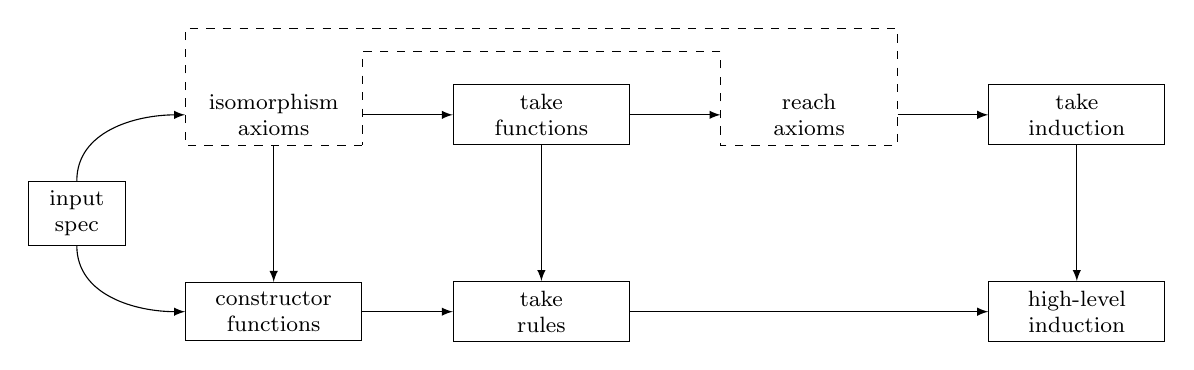
\begin{tikzpicture}
  [ axiom/.style={rectangle, text width=2cm, text centered, font=\footnotesize}
  , proof/.style={rectangle, text width=2cm, text centered, font=\footnotesize, draw}
  , >=latex]
  \node (0) at (-2.5, 1.25) [rectangle, text width=1cm, text centered, font=\footnotesize, draw] {input\\spec};
  \node (1) at (0.0, 2.5) [axiom] {isomorphism\\axioms};
  \node (2) at (3.4, 2.5) [proof] {take\\functions};
  \node (3) at (6.8, 2.5) [axiom] {reach\\axioms};
  \node (4) at (10.2, 2.5) [proof] {take\\induction};
  \node (5) at (0.0, 0.0) [proof] {constructor\\functions};
  \node (6) at (3.4, 0.0) [proof] {take\\rules};
  \node (7) at (10.2, 0.0) [proof] {high-level\\induction};
  \draw [->] (0.north) to [out=90, in=180] (1.west);
  \draw [->] (1) -- (2);
  \draw [->] (2) -- (3);
  \draw [->] (3) -- (4);
  \draw [->] (0.south) to [out=270, in=180] (5.west);
  \draw [->] (1) -- (5);
  \draw [->] (5) -- (6);
  \draw [->] (2) -- (6);
  \draw [->] (6) -- (7);
  \draw [->] (4) -- (7);
  \draw [dashed]
    (1.south east) -- (1.south west) -- (1.north west) --
    (1.west |- 0,3.6) -- (3.east |- 0,3.6) -- (3.south east) -- (3.south west) --
    (3.west |- 0,3.3) -- (1.east |- 0,3.3) -- (1.south east) -- cycle;
\end{tikzpicture}
\end{singlespace}
\end{center}
\caption{Domain package implementation schematic}
\label{fig:universal-schematic}
\end{figure}

The axiomatic \textsc{Domain} package generates two kinds of axioms: First, isomorphism axioms state that the \isa{rep} and \isa{abs} functions for each new type are each other's inverses. Second, the reach axiom for each type states a low-level induction rule, asserting that the least upper bound of a chain of take functions is the identity. The remainder of this section will show how these axioms are derived as theorems, using a lazy list datatype as an example to help explain the process.
%
\begin{isacode}
domain 'a llist = LNil | LCons (lazy "'a") (lazy "'a llist")
\end{isacode}

\subsection{Proving the isomorphism theorems}
\label{sec:universal-package-iso}

To construct a domain isomorphism for the lazy list type, information about data constructors is irrelevant; all we need is the domain equation \isa{'a llist} $\cong$ \isa{one \<oplus> ('a\<lifted> \<otimes>} \isa{'a llist\<lifted>)}. Solving this domain equation is a three-step process: The definitional \textsc{Domain} package first defines a deflation combinator, then uses the deflation to define the \isa{'a llist} type, and finally defines the isomorphism functions.

\paragraph{Defining deflation combinators.}
%
The first step is to define a deflation combinator \isa{llist_defl :: udom defl \<rightarrow> udom defl} that models the lazy list type constructor. The deflation combinator is determined by the domain equation that type \isa{'a llist} must satisfy:
%
\begin{isacode}
'a llist \<cong> one \<oplus> ('a\<lifted> \<otimes> 'a llist\<lifted>)
\end{isacode}

The definition of \isa{llist_defl} will refer to the deflation combinator of each type constructor mentioned on the right-hand side of this domain equation. To keep track of the correspondence between type constructors and deflation combinators, the \textsc{Domain} package maintains an extensible list of theorems with the \isa{[domain_defl_simps]} attribute. The initial set of these rules is shown in Fig.~\ref{fig:universal-domain-defl-simps}.

\begin{figure}
\begin{isacode}
lemma [domain_defl_simps]:
  "DEFL('a \<rightarrow> 'b) = cfun_defl\<cdot>DEFL('a)\<cdot>DEFL('b)"
  "DEFL('a \<oplus> 'b) = ssum_defl\<cdot>DEFL('a)\<cdot>DEFL('b)
  "DEFL('a \<otimes> 'b) = sprod_defl\<cdot>DEFL('a)\<cdot>DEFL('b)"
  "DEFL('a \<times> 'b) = prod_defl\<cdot>DEFL('a)\<cdot>DEFL('b)"
  "DEFL('a\<^sub>\<bottom>) = u_defl\<cdot>DEFL('a)"
  "DEFL(('a)\<sharp>) = upper_defl\<cdot>DEFL('a)"
  "DEFL(('a)\<flat>) = lower_defl\<cdot>DEFL('a)"
  "DEFL(('a)\<natural>) = convex_defl\<cdot>DEFL('a)"
\end{isacode}
\caption{Extensible set of rules with the \isa{domain_defl_simps} attribute}
\label{fig:universal-domain-defl-simps}
\end{figure}

Using \isa{domain_defl_simps}, the \textsc{Domain} package produces the recursive specification of \isa{llist_defl} shown below as \isa{llist_defl_unfold}. The actual non-recursive definition of \isa{llist_defl}, using the least fixed point combinator \isa{fix}, is created using the same machinery employed by the \textsc{Fixrec} package; \isa{llist_defl_unfold} is then derived from the non-recursive definition as a theorem.
%
\begin{isacode}
theorem llist_defl_unfold:
  "llist_defl\<cdot>t = ssum_defl\<cdot>DEFL(one)\<cdot>(sprod_defl\<cdot>(u_defl\<cdot>t)\<cdot>(u_defl\<cdot>(llist_defl\<cdot>t)))"
\end{isacode}

\paragraph{Defining representable domains from deflations.}
%
The second step is to use \isa{llist_defl} to define the actual \isa{'a llist} type. In Sections \ref{sec:definitional-alg-combinators} and \ref{sec:universal-representable}, the aim was to build algebraic deflations of type \isa{udom defl} to correspond with pre-existing cpo types. Now, we need to do the converse: Given a deflation of type \isa{udom defl}, we must define the corresponding cpo. We can accomplish this with the help of the \textsc{Cpodef} package.

The first step in defining a new cpo type with \textsc{Cpodef} is to determine a subset of values of the old cpo type. We define the \isa{defl_set} function for this purpose: It produces the image set of any deflation \isa{t}, defined as the set of fixed points of \isa{cast\<cdot>t}.
\vspace{-22pt} % FUDGE
\indexdef{defl_set}
\begin{isacode}
definition defl_set :: "'a defl \<Rightarrow> 'a set"
  where "defl_set t = {x. cast\<cdot>t\<cdot>x = x}"
\end{isacode}
%
Now we can define \isa{'a llist} as a pointed cpo, isomorphic to the image set of the deflation \isa{llist_defl\<cdot>DEFL('a)}.
%
\begin{isacode}
pcpodef (open) 'a llist = "defl_set (llist_defl\<cdot>DEFL('a))"
\end{isacode}
%
The \textsc{Cpodef} package generates two proof obligations: First, that membership in the given set is admissible, and also that the given set contains \isa{\<bottom>}. Both of these properties hold for any application of \isa{defl_set}.

\indexthm{adm_defl_set}
\begin{isacode}
lemma adm_defl_set: "adm (\<lambda>x. x \<in> defl_set t)"
\end{isacode}
\unmedskip
\indexthm{defl_set_bottom}
\begin{isacode}
lemma defl_set_bottom: "\<bottom> \<in> defl_set t"
\end{isacode}

The \isa{pcpodef} command only proves that type \isa{'a llist} is a \isa{pcpo}; we still need to provide an instantiation of the \isa{"domain"} class. This instantiation requires definitions of \isa{emb}, \isa{prj}, and \isa{defl}, which are defined as follows:
%
\begin{isacode}
instantiation llist :: ("domain") "domain"
begin
  definition "(emb :: 'a llist \<rightarrow> udom) \<equiv> (\<Lambda> x. Rep_llist x)"
  definition "(prj :: udom \<rightarrow> 'a llist) \<equiv>
      (\<Lambda> x. Abs_llist (cast\<cdot>(llist_defl\<cdot>DEFL('a))\<cdot>x))"
  definition "defl \<equiv> (\<lambda>(_ :: 'a llist itself). llist_defl\<cdot>DEFL('a))"
  instance ...
end
\end{isacode}
%
The instance proof requires us to show that \isa{emb} and \isa{prj} are an ep-pair, and also that the composition \isa{emb oo prj} is equal to \isa{cast\<cdot>DEFL('a llist)}. Instead of repeating this proof for each new domain definition, we employ a generic lemma that proves the \isa{OFCLASS} predicate, in the style of the lemmas used to implement \textsc{Cpodef}.
%
\indexthm{typedef_domain_class}
\begin{isacode}
lemma typedef_domain_class:
  fixes Rep :: "'a::pcpo \<Rightarrow> udom"
  fixes Abs :: "udom \<Rightarrow> 'a::pcpo"
  fixes t :: "udom defl"
  assumes type: "type_definition Rep Abs (defl_set t)"
  assumes below: "below \<equiv> (\<lambda>x y. Rep x \<sqsubseteq> Rep y)"
  assumes emb: "emb \<equiv> (\<Lambda> x. Rep x)"
  assumes prj: "prj \<equiv> (\<Lambda> x. Abs (cast\<cdot>t\<cdot>x))"
  assumes defl: "defl \<equiv> (\<lambda>(_ :: 'a itself). t)"
  shows "OFCLASS('a, domain_class)"
\end{isacode}
%
The assumptions \isa{type} and \isa{below} in this rule can be satisfied by theorems generated by \textsc{Cpodef}; the other assumptions are simply the definitions from the \isa{"domain"} class instantiation.

After proving the class instance, we can extend \isa{domain_defl_simps} with a new rule for the lazy list type constructor; this rule follows immediately from the definition of \isa{defl} for lazy lists.
%
\indexthmx{DEFL_llist}
\begin{isacode}
theorem DEFL_llist [domain_defl_simps]: "DEFL('a llist) = llist_defl\<cdot>DEFL('a)"
\end{isacode}

This entire process of defining a representable domain from a deflation is automated with the \textsc{Domaindef} package, which is built as a thin layer on top of the \textsc{Cpodef} package. \textsc{Domaindef} is called internally by the definitional \textsc{Domain} package, and it is also available as a user-level command. Unlike \textsc{Cpodef}, it is completely automatic; no additional proof obligations are needed.
%
\begin{isacode}
domaindef 'a llist = "llist_defl\<cdot>DEFL('a)"
\end{isacode}
%
The above \isa{domaindef} command defines type \isa{'a llist}, proves a \isa{"domain"} class instance, and adds theorem \isa{DEFL_llist} to \isa{domain_defl_simps}.

\paragraph{Constructing isomorphism functions as coercions.}

The third step is to actually construct the desired domain isomorphism, by defining continuous \isa{rep} and \isa{abs} functions and proving that they are each other's inverses.

For any representable domains \isa{'a} and \isa{'b}, composing \isa{emb :: 'a \<rightarrow> udom} with \isa{prj :: udom \<rightarrow> 'b} yields a \emph{coercion} \isa{prj oo emb :: 'a \<rightarrow> 'b}. If \isa{DEFL('a) \<sqsubseteq> DEFL('b)}, then the coercions from \isa{'a} to \isa{'b} and back form an ep-pair. If \isa{DEFL('a) = DEFL('b)}, then the coercions from \isa{'a} to \isa{'b} and back form a continuous isomorphism. The \textsc{Domain} package uses this fact to define the \isa{rep} and \isa{abs} functions for each new domain, and show that they form a continuous isomorphism.

\indexdefx{llist_rep}
\begin{isacode}
definition llist_rep :: "'a llist \<rightarrow> one \<oplus> ('a\<lifted> \<otimes> 'a llist\<lifted>)"
  where "llist_rep \<equiv> prj oo emb"
\end{isacode}
\unmedskip
\indexdefx{llist_abs}
\begin{isacode}
definition llist_abs :: "one \<oplus> ('a\<lifted> \<otimes> 'a llist\<lifted>) \<rightarrow> 'a llist"
  where "llist_abs \<equiv> prj oo emb"
\end{isacode}

Before we can prove that \isa{llist_rep} and \isa{llist_abs} are a continuous isomorphism, we must prove that the types they coerce between are represented by the same deflation. Theorem \isa{DEFL_eq_llist} is easily proved using \isa{domain_defl_simps} together with \isa{llist_defl_unfold}.
%
\indexthmx{DEFL_eq_llist}
\begin{isacode}
theorem DEFL_eq_llist: "DEFL('a llist) = DEFL(one \<oplus> ('a\<lifted> \<otimes> 'a llist\<lifted>))"
\end{isacode}

Using \isa{DEFL_eq_llist}, the definitional \textsc{Domain} package can \emph{prove} that \isa{llist_abs} and \isa{llist_rep} are an isomorphism---in the axiomatic \textsc{Domain} package, \isa{llist.abs_iso} and \isa{llist.rep_iso} would have been declared as axioms.
%
\indexthmx{llist.abs_iso}
\begin{isacode}
theorem llist.abs_iso: "llist_rep\<cdot>(llist_abs\<cdot>x) = x"
\end{isacode}
\unmedskip
\indexthmx{llist.rep_iso}
\begin{isacode}
theorem llist.rep_iso: "llist_abs\<cdot>(llist_rep\<cdot>y) = y"
\end{isacode}
%
Theorem \isa{llist.abs_iso} is proved by instantiating lemma \isa{domain_abs_iso} from the library with \isa{DEFL_eq_llist} and the definitions of \isa{llist_abs} and \isa{llist_rep}.
%
\indexthm{domain_abs_iso}
\begin{isacode}
lemma domain_abs_iso:
  fixes abs :: "'a \<rightarrow> 'b" and rep :: "'b \<rightarrow> 'a"
  assumes DEFL: "DEFL('b) = DEFL('a)"
  assumes abs_def: "abs \<equiv> prj oo emb"
  assumes rep_def: "rep \<equiv> prj oo emb"
  shows "rep\<cdot>(abs\<cdot>x) = x"
\end{isacode}
%
Theorem \isa{llist_rep_iso} is proved using a similar rule, \isa{domain_rep_iso}, which concludes \isa{abs\<cdot>(rep\<cdot>y) = y} from the same assumptions.

\subsection{Proving the reach lemma}
\label{sec:universal-package-reach}

After the new definitional \textsc{Domain} package code constructs the isomorphism, the take-function component (described in Chapter~\ref{ch:domain}) defines \isa{llist_take}, and proves some theorems (listed in Fig.~\ref{fig:universal-llist-take}). Now the definitional \textsc{Domain} package needs to prove the reach lemma, which states that the least upper bound of the chain \isa{llist_take} is the identity function.

\begin{figure}
\begin{isacode}
theorem llist.take_def:
  "llist_take \<equiv> (\<lambda>n. iterate n\<cdot>
    (\<Lambda> g. llist_abs oo ssum_map\<cdot>ID\<cdot>(sprod_map\<cdot>ID\<cdot>(u_map\<cdot>g)) oo llist_rep)\<cdot>\<bottom>)"
\end{isacode}
\unmedskip
\begin{isacode}
theorem llist.take_0: "llist_take 0 = \<bottom>"
\end{isacode}
\unmedskip
\begin{isacode}
theorem llist.take_Suc: "llist_take (Suc n) =
  llist_abs oo ssum_map\<cdot>ID\<cdot>(sprod_map\<cdot>ID\<cdot>(u_map\<cdot>(llist_take n))) oo llist_rep"
\end{isacode}
\unmedskip
\begin{isacode}
theorem llist.chain_take: "chain llist_take"
\end{isacode}
\unmedskip
\begin{isacode}
theorem llist.deflation_take: "deflation (llist_take n)"
\end{isacode}
\caption{Definition and basic properties of \isa{llist_take} function}
\label{fig:universal-llist-take}
\end{figure}

As an integrated part of the process of deriving the reach lemma, the definitional \textsc{Domain} package also performs the necessary steps to allow indirect recursion with \isa{llist} in later domain definitions. This involves defining a map function \isa{llist_map}, proving a few theorems about it, and adding those theorems to the appropriate databases.

The overall process can be broken down into three main steps: First, define the map function. Second, prove the identity law for the map function, by establishing a relationship between the map function and the deflation combinator. Third, prove the reach lemma by relating the take function to the map function.

\paragraph{Defining the map function.}

The \textsc{Domain} package defines the map function \isa{llist_map} of type \isa{('a \<rightarrow> 'a) \<rightarrow> 'a llist \<rightarrow> 'a llist}.\footnote{The most general type of \isa{llist_map} is actually \isa{('a \\<rightarrow> 'b) \\<rightarrow> 'a llist \\<rightarrow> 'b llist}. However, the current implementation uses the more restrictive type scheme because it works without modification for contravariant types. Generalizing the types of map functions is planned as future work.} It generates a recursive specification from a combination of other map functions, based on the structure of the type \isa{one \<oplus> ('a\<lifted> \<otimes> 'a llist\<lifted>)}. As with the deflation combinator, the actual fixed point definition is handled by \textsc{Fixrec}-style machinery.
%
\begin{isacode}
theorem llist_map_unfold:
  "llist_map\<cdot>f = llist_abs oo
    ssum_map\<cdot>ID\<cdot>(sprod_map\<cdot>(u_map\<cdot>f)\<cdot>(u_map\<cdot>(llist_map\<cdot>f))) oo llist_rep"
\end{isacode}

At this point the \textsc{Domain} package proves one of the rules needed for later indirect-recursive definitions, which states that \isa{llist_map} preserves deflations. Theorem \isa{deflation_llist_map} is proved by fixed point induction, using the pre-existing \isa{domain_deflation} rules; it is then added to the \isa{domain_deflation} rule database.
%
\begin{isacode}
theorem deflation_llist_map [domain_deflation]:
  "deflation f \<Longrightarrow> deflation (llist_map\<cdot>f)"
\end{isacode}

\paragraph{Proving the identity law.}

The other property that we must prove about \isa{llist_map} is the identity law, \isa{llist_map\<cdot>ID = ID}. To prove this property, the \textsc{Domain} package exploits the similarities in the recursive definitions of \isa{llist_map} and the \isa{llist_defl}. The relationship between the two is formalized in a binary relation called \isa{isodefl}, which states that the given function \isa{f} is ``isomorphic'' in some sense to the algebraic deflation \isa{t}.

\begin{isacode}
definition isodefl :: "('a::domain \<rightarrow> 'a) \<Rightarrow> udom defl \<Rightarrow> bool"
  where "isodefl f t = (cast\<cdot>t = emb oo f oo prj)"
\end{isacode}

The \textsc{Domain} package maintains a database of theorems relating map functions to their corresponding deflation combinators, using the attribute \isa{[domain_isodefl]}. The initial contents of this database are shown in Fig.~\ref{fig:universal-domain-isodefl}.

\begin{figure}
\begin{isacode}
lemma [domain_isodefl]:
  "isodefl (ID :: 'a \<rightarrow> 'a) DEFL('a)"
  "\<lbrakk>isodefl f1 t1; isodefl f2 t2\<rbrakk> \<Longrightarrow> isodefl (cfun_map\<cdot>f1\<cdot>f2) (cfun_defl\<cdot>t1\<cdot>t2)"
  "\<lbrakk>isodefl f1 t1; isodefl f2 t2\<rbrakk> \<Longrightarrow> isodefl (ssum_map\<cdot>f1\<cdot>f2) (ssum_defl\<cdot>t1\<cdot>t2)"
  "\<lbrakk>isodefl f1 t1; isodefl f2 t2\<rbrakk> \<Longrightarrow> isodefl (sprod_map\<cdot>f1\<cdot>f2) (sprod_defl\<cdot>t1\<cdot>t2)"
  "\<lbrakk>isodefl f1 t1; isodefl f2 t2\<rbrakk> \<Longrightarrow> isodefl (prod_map\<cdot>f1\<cdot>f2) (prod_defl\<cdot>t1\<cdot>t2)"
  "isodefl f t \<Longrightarrow> isodefl (u_map\<cdot>f) (u_defl\<cdot>t)"
  "isodefl f t \<Longrightarrow> isodefl (upper_map\<cdot>f) (upper_defl\<cdot>t)"
  "isodefl f t \<Longrightarrow> isodefl (lower_map\<cdot>f) (lower_defl\<cdot>t)"
  "isodefl f t \<Longrightarrow> isodefl (convex_map\<cdot>f) (convex_defl\<cdot>t)"
\end{isacode}
\caption{Extensible set of rules with the \isa{domain_isodefl} attribute}
\label{fig:universal-domain-isodefl}
\end{figure}

Now the \textsc{Domain} package must prove a similar \isa{domain_isodefl} rule for the lazy list type:
%
\begin{isacode}
theorem isodefl_llist [domain_isodefl]:
  "isodefl f t \<Longrightarrow> isodefl (llist_map\<cdot>f) (llist_defl\<cdot>t)"
\end{isacode}
%
The proof proceeds by a form of parallel fixed point induction: After unfolding the definitions of \isa{llist_map} and \isa{llist_defl} to reveal the underlying fixed point combinators, rule \isa{parallel_fix_ind} can be applied.
%
\begin{isacode}
lemma parallel_fix_ind:
  "\<lbrakk>adm (\<lambda>x. P (fst x) (snd x)); P \<bottom> \<bottom>; \<And>x y. P x y \<Longrightarrow> P (F\<cdot>x) (G\<cdot>y)\<rbrakk>
    \<Longrightarrow> P (fix\<cdot>F) (fix\<cdot>G)"
\end{isacode}
%
After discharging the admissibility check and the base case \isa{isodefl \<bottom> \<bottom>}, the final subgoal is nontrivial:

\begin{isacode}
goal (1 subgoal):
 1. \<And>x y. \<lbrakk>isodefl f t; isodefl x y\<rbrakk>
\end{isacode}
\pagebreak
\begin{isacode}
          \<Longrightarrow> isodefl
              (llist_abs oo
               ssum_map\<cdot>ID\<cdot>(sprod_map\<cdot>(u_map\<cdot>f)\<cdot>(u_map\<cdot>x)) oo llist_rep)
              (ssum_defl\<cdot>DEFL(one)\<cdot>(sprod_defl\<cdot>(u_defl\<cdot>t)\<cdot>(u_defl\<cdot>y)))
\end{isacode}
%
This last subgoal is solved by repeatedly applying rules from the \isa{domain_isodefl} database, along with one extra rule to handle the occurrences of \isa{llist_abs} and \isa{llist_rep}:
%
\begin{isacode}
theorem llist.isodefl_abs_rep:
  "isodefl f t \<Longrightarrow> isodefl (llist_abs oo f oo llist_rep) t"
\end{isacode}
%
A similar theorem holds for any \isa{rep} and \isa{abs} functions defined as coercions between isomorphic types.

Once theorem \isa{isodefl_llist} has been proven, the \textsc{Domain} package uses lemmas \isa{isodefl_DEFL_imp_ID} and \isa{DEFL_llist} to derive the identity law for \isa{llist_map} as a corollary.
%
\indexthm{isodefl_DEFL_imp_ID}
\begin{isacode}
lemma isodefl_DEFL_imp_ID: "isodefl f DEFL('a) \<Longrightarrow> f = ID"
\end{isacode}
\unmedskip
\indexthmx{llist_map_ID}
\begin{isacode}
theorem llist_map_ID [domain_map_ID]: "llist_map\<cdot>ID = ID"
\end{isacode}
%
Once proved, \isa{llist_map_ID} is added to the \isa{domain_map_ID} database (introduced in Chapter~\ref{ch:domain}) for use in later domain definitions.

\paragraph{Relating the map and take functions.}

In the final step, the reach lemma can be derived from the identity law of \isa{llist_map}, by taking advantage of similarities in the definitions of \isa{llist_take} and \isa{llist_map}.
%
\begin{isacode}
theorem llist.lub_take: "(\<Squnion>n. llist_take n) = ID"
\end{isacode}
%
The proof begins by applying transitivity with \isa{llist_map_ID}, yielding the subgoal 
\isa{(\<Squnion>n. llist_take n)} \isa{= llist_map\<cdot>ID}. After unfolding the definitions of \isa{llist_take}, \isa{llist_map}, and the fixed point combinator \isa{fix}, both sides of the equality have the form \isa{(\<Squnion>n. iterate\<cdot>f\<cdot>\<bottom>)}. Rewriting with \isa{domain_map_ID} rules can finish the proof.

\subsection{User-visible changes}

In \HOLCF{11}, the \textsc{Domain} package operates in definitional mode by default. For backward compatibility, the axiomatic mode is still available using the \isa{domain} \isa{(unsafe)} command. The primary user-visible difference between the two modes is which type classes they use: In definitional mode, type parameters and other constructor argument types must be in class \isa{"domain"}; newly-defined datatypes are also made instances of the \isa{"domain"} class. In contrast, the axiomatic mode uses the \isa{pcpo} class throughout. Even with this change, most HOLCF user theories work without modification, because the default sort has also changed from \isa{pcpo} to \isa{"domain"}.

The other user-visible change is the new support for indirect recursion. After defining type \isa{'a llist} with the definitional \textsc{Domain} package, users can define other datatypes using indirect recursion with \isa{llist}, such as this datatype of trees:
%
\begin{isacode}
domain 'a tree = Leaf (lazy "'a") | Node (lazy "'a tree llist")
\end{isacode}
%
In axiomatic mode, however, the \textsc{Domain} package does not generate map functions, and does not configure indirect recursion to work with new datatypes.

\section{Unpointed predomains}
\label{sec:universal-predomain}

Prior to \HOLCF{11}, \isa{pcpo} has always been the default sort; any type variables mentioned in HOLCF theories were assumed to be in class \isa{pcpo} by default. However, the class \isa{cpo}, which is a superclass of \isa{pcpo} that does not require a bottom element, is also useful in some cases. Various theory developments based on \HOLCF{99} have made use of the \isa{cpo} class \cite{hol+lcf, mueller98thesis}. With \HOLCF{11} switching from \isa{pcpo} to the \isa{"domain"} class, what should be done with these theories that use class \isa{cpo}? There is a need for an unpointed variant of class \isa{"domain"} in \HOLCF{11}.

To fill this need, we introduce a class of \emph{predomains}. A predomain is a cpo that, when lifted, becomes a representable domain. More precisely, while \isa{'a::"domain"} means that type \isa{'a} can be embedded into \isa{udom}, \isa{'a::predomain} means that type \isa{'a\<^sub>\<bottom>} can be embedded into \isa{udom\<^sub>\<bottom>}.

\indexdef{class predomain_syn}
\begin{isacode}
class predomain_syn = cpo +
  fixes liftemb :: "'a\<^sub>\<bottom> \<rightarrow> udom\<^sub>\<bottom>"
  fixes liftprj :: "udom\<^sub>\<bottom> \<rightarrow> 'a\<^sub>\<bottom>"
  fixes liftdefl :: "'a itself \<Rightarrow> (udom\<^sub>\<bottom>) defl"
\end{isacode}
\unmedskip
\indexdef{class predomain}
\begin{isacode}
class predomain = predomain_syn +
  assumes predomain_ep: "ep_pair liftemb liftprj"
  assumes cast_liftdefl: "cast\<cdot>(liftdefl TYPE('a)) = liftemb oo liftprj"
\end{isacode}
%
We also define \isa{LIFTDEFL('a)} as a convenient abbreviation for \isa{liftdefl TYPE('a)}.

Shortly we will redefine the \isa{"domain"} type class to make it into a subclass of \isa{predomain}. But in order to do that, we need a function for creating deflations on \isa{udom\<^sub>\<bottom>} out of deflations on \isa{udom}.

\indexdef{liftdefl_of}
\begin{isacode}
definition liftdefl_of :: "udom defl \<rightarrow> (udom\<^sub>\<bottom>) defl"
  where "liftdefl_of = defl_fun1 ID ID u_map"
\end{isacode}
\unmedskip
\indexthm{cast_liftdefl_of}
\begin{isacode}
lemma cast_liftdefl_of: "cast\<cdot>(liftdefl_of\<cdot>t) = u_map\<cdot>(cast\<cdot>t)"
\end{isacode}
%
We now extend the \isa{"domain"} type class by adding \isa{predomain_syn} as a superclass, along with a few class assumptions stating that \isa{liftemb}, \isa{liftprj}, and \isa{liftdefl} are defined in a standard way.
%
\begin{isacode}
class "domain" = predomain_syn + pcpo +
  fixes emb :: "'a \<rightarrow> udom"
  fixes prj :: "udom \<rightarrow> 'a"
  fixes defl :: "'a itself \<Rightarrow> udom defl"
  assumes ep_pair_emb_prj: "ep_pair emb prj"
  assumes cast_DEFL: "cast\<cdot>(defl TYPE('a)) = emb oo prj"
  assumes liftemb_eq: "liftemb = u_map\<cdot>emb"
  assumes liftprj_eq: "liftprj = u_map\<cdot>prj"
  assumes liftdefl_eq: "liftdefl TYPE('a) = liftdefl_of\<cdot>(defl TYPE('a))"
\end{isacode}
%
It is then a simple matter to prove the subclass relationship \isa{"domain" \<subseteq> predomain}, by showing that the definitions of \isa{liftemb}, \isa{liftprj}, and \isa{liftdefl} specified by the \isa{"domain"} class satisfy the \isa{predomain} axioms.

\paragraph{Domain class instance for lifted cpo.} Now we define a new \isa{"domain"} class instance for the lifted cpo type \isa{'a\<^sub>\<bottom>}, so that the type argument \isa{'a} only needs to be a \isa{predomain}. To implement this class instance, we need a new variant of the deflation combinator \isa{u_defl} whose argument type is \isa{(udom\<^sub>\<bottom>) defl} instead of \isa{udom defl}.
%
\indexdef{u_liftdefl}
\begin{isacode}
definition u_liftdefl :: "(udom\<^sub>\<bottom>) defl \<rightarrow> udom defl"
  where "u_liftdefl = defl_fun1 u_emb u_prj ID"
\end{isacode}
\unmedskip
\indexthm{cast_u_liftdefl}
\begin{isacode}
lemma cast_u_liftdefl: "cast\<cdot>(u_liftdefl\<cdot>t) = u_emb oo cast\<cdot>t oo u_prj"
\end{isacode}
%
Here \isa{u_emb :: udom\<^sub>\<bottom> \<rightarrow> udom} and \isa{u_prj :: udom \<rightarrow> udom\<^sub>\<bottom>} are the ep-pair provided by the universal domain library---the same functions are used to define \isa{u_defl}. The two deflation combinators are related by the following theorem:
%
\indexthm{u_liftdefl_liftdefl_of}
\begin{isacode}
lemma u_liftdefl_liftdefl_of: "u_liftdefl\<cdot>(liftdefl_of\<cdot>t) = u_defl\<cdot>t"
\end{isacode}
%
This means that although \isa{DEFL('a\<^sub>\<bottom>) = u_liftdefl\<cdot>LIFTDEFL('a)} by definition, it is also still equal to \isa{u_defl\<cdot>DEFL('a)} for any \isa{'a} in class \isa{"domain"}, just as it was defined before.
%
\begin{isacode}
instantiation u :: (predomain) "domain"
begin
  definition "(emb :: 'a\<^sub>\<bottom> \<rightarrow> udom) = u_emb oo liftemb"
  definition "(prj :: udom \<rightarrow> 'a\<^sub>\<bottom>) = liftprj oo u_prj"
  definition "defl (_ :: ('a\<^sub>\<bottom>) itself) = u_liftdefl\<cdot>LIFTDEFL('a)"
  ...
end
\end{isacode}
%
The functions \isa{liftemb}, \isa{liftprj}, and \isa{liftdefl} are all defined exactly as required by the \isa{"domain"} class axioms. The other \isa{"domain"} class axioms about \isa{emb}, \isa{prj}, and \isa{defl} follow from the \isa{predomain} class axioms on type \isa{'a}.

\paragraph{Predomain class instance for cartesian product.}

The goal here is to create a \isa{predomain} instance for products, such that the product of two predomains is again a predomain. To do this, we must create an ep-pair from type \isa{('a \<times> 'b)\<^sub>\<bottom>} into \isa{udom\<^sub>\<bottom>}. To define the embedding and projection, we make use of an isomorphism between type \isa{('a \<times> 'b)\<^sub>\<bottom>} and the strict product \isa{'a\<^sub>\<bottom> \<otimes> 'b\<^sub>\<bottom>}.

\indexdef{encode_prod_u}
\begin{isacode}
definition encode_prod_u :: "('a \<times> 'b)\<^sub>\<bottom> \<rightarrow> 'a\<^sub>\<bottom> \<otimes> 'b\<^sub>\<bottom>"
  where "encode_prod_u = (\<Lambda>(up\<cdot>(x, y)). (:up\<cdot>x, up\<cdot>y:))"
\end{isacode}
\unmedskip
\indexdef{decode_prod_u}
\begin{isacode}
definition decode_prod_u :: "'a\<^sub>\<bottom> \<otimes> 'b\<^sub>\<bottom> \<rightarrow> ('a \<times> 'b)\<^sub>\<bottom>"
  where "decode_prod_u = (\<Lambda>(:up\<cdot>x, up\<cdot>y:). up\<cdot>(x, y))"
\end{isacode}

The embedding can now be done in multiple steps: Starting with a value of type \isa{('a \<times> 'b)\<^sub>\<bottom>}, first apply \isa{encode_prod_u} to get a strict pair of type \isa{'a\<^sub>\<bottom> \<otimes> 'b\<^sub>\<bottom>}. Second, map \isa{liftemb} over each component of the strict pair to get another pair of type \isa{udom\<^sub>\<bottom> \<otimes> udom\<^sub>\<bottom>}. Third, apply \isa{decode_prod_u} to convert this to type \isa{(udom \<times> udom)\<^sub>\<bottom>}. Finally, map the embedding function for type \isa{udom \<times> udom} over the lifted cpo to get a value of type \isa{udom\<^sub>\<bottom>}. The projection uses the same process in reverse. We then define the deflation combinator \isa{prod_liftdefl} to correspond with the composition of these embedding and projection functions.

\indexdef{prod_liftdefl}
\begin{isacode}
definition prod_liftdefl :: "(udom\<^sub>\<bottom>) defl \<rightarrow> (udom\<^sub>\<bottom>) defl \<rightarrow> (udom\<^sub>\<bottom>) defl"
  where "prod_liftdefl = defl_fun2 (u_map\<cdot>prod_emb oo decode_prod_u)
    (encode_prod_u oo u_map\<cdot>prod_prj) sprod_map"
\end{isacode}
\unmedskip
\indexthm{cast_prod_liftdefl}
\begin{isacode}
lemma cast_prod_liftdefl:
  "cast\<cdot>(prod_liftdefl\<cdot>a\<cdot>b) = (u_map\<cdot>prod_emb oo decode_prod_u) oo
    sprod_map\<cdot>(cast\<cdot>a)\<cdot>(cast\<cdot>b) oo (encode_prod_u oo u_map\<cdot>prod_prj)"
\end{isacode}
\unmedskip
\begin{isacode}
instantiation prod :: (predomain, predomain) predomain
begin
  definition "liftemb = (u_map\<cdot>prod_emb oo decode_prod_u)
      oo (sprod_map\<cdot>liftemb\<cdot>liftemb oo encode_prod_u)"
  definition "liftprj = (decode_prod_u oo sprod_map\<cdot>liftprj\<cdot>liftprj)
      oo (encode_prod_u oo u_map\<cdot>prod_prj)"
  definition "liftdefl (_ :: ('a \<times> 'b) itself) =
      prod_liftdefl\<cdot>LIFTDEFL('a)\<cdot>LIFTDEFL('b)"
  instance ...
end
\end{isacode}
%
Although the definitions may look complex, the \isa{predomain} instance proof is still relatively simple. Showing \isa{ep_pair liftemb liftprj} merely requires a few extra applications of rules from Fig.~\ref{fig:universal-ep-pair-lemmas}.
%
\begin{isacode}
instantiation prod :: ("domain", "domain") "domain"
begin
  definition "(emb :: 'a \<times> 'b \<rightarrow> udom) = prod_emb oo prod_map\<cdot>emb\<cdot>emb"
  definition "(prj :: udom \<rightarrow> 'a \<times> 'b) = prod_map\<cdot>prj\<cdot>prj oo prod_prj"
  definition "defl (_ :: ('a \<times> 'b) itself) = prod_defl\<cdot>DEFL('a)\<cdot>DEFL('b)"
  instance ...
end
\end{isacode}
%
On the other hand, the \isa{"domain"} instance proof requires more work than one might expect. The reason is that unlike any other \isa{"domain"} class instantiation, the product type does not have \isa{liftemb}, \isa{liftprj}, and \isa{liftdefl} defined exactly as specified by the \isa{"domain"} class axioms. Fortunately, \isa{liftemb = u_map\<cdot>emb} and \isa{liftprj = u_map\<cdot>prj} can be proved without too much trouble by case analysis on their inputs. Also, \isa{LIFTDEFL('a \<times> 'b) = liftdefl_of\<cdot>DEFL('a \<times> 'b)} can be proved using the injectivity of \isa{cast}, by showing that \isa{cast\<cdot>LIFTDEFL('a \<times> 'b) = cast\<cdot>(liftdefl_of\<cdot>DEFL('a \<times> 'b))}.

\paragraph{Other class instances.} Other \isa{predomain} class instances can be defined in a similar way to the product type. For example, with the Isabelle/HOL disjoint sum type, an isomorphism can be defined between type \isa{('a + 'b)\<^sub>\<bottom>} and the strict sum \isa{'a\<^sub>\<bottom> \<oplus> 'b\<^sub>\<bottom>}. This can be used to show that the disjoint sum of two predomains is again a predomain.

Another isomorphism that was noted back in Chapter~\ref{ch:holcf} is between type \isa{'a discr\<^sub>\<bottom>} and \isa{'a lift}. This is used to make \isa{'a discr} an instance of class \isa{predomain}, for any countable type \isa{'a}.

The last new class instance of note is for the continuous function type. To show that type \isa{'a \<rightarrow> 'b} is in class \isa{pcpo}, \isa{'b} must be a \isa{pcpo}, but \isa{'a} only needs to be in class \isa{cpo}. How can we get a similar instance for the \isa{"domain"}  and \isa{predomain} classes? In order to prove this class instance, we can define a type \isa{'a \<rightarrow>! 'b}, which is the \emph{strict function space} from \isa{'a} to \isa{'b}.
%
\begin{isacode}
pcpodef (open) ('a, 'b) sfun (infixr "\<rightarrow>!" 0) = "{f :: 'a \<rightarrow> 'b. f\<cdot>\<bottom> = \<bottom>}"
\end{isacode}
%
For an unpointed \isa{'a} and pointed \isa{'b}, type \isa{'a \<rightarrow> 'b} is isomorphic to the strict function type \isa{'a\<^sub>\<bottom> \<rightarrow>! 'b}. This can then be used to obtain the desired class instance for continuous functions.

\paragraph{Domain package support for predomains.} Some minor changes to the \textsc{Domain} package were necessary to add support for predomains. Two new features were implemented. First, lazy constructor arguments are now permitted to be in class \isa{predomain}. (Strict constructor arguments are still required to be in class \isa{"domain"}.) For example, we can define the following type of lazy lists of natural numbers, where the elements have the unpointed type \isa{nat discr}:
%
\begin{isacode}
domain natlist = nil | cons (lazy "nat discr") (lazy "natlist")
\end{isacode}
%
The second feature is that datatypes can now have type parameters in class \isa{predomain}. For example, we can define a variation of the lazy list datatype that allows unpointed predomain element types:
%
\begin{isacode}
domain ('a::predomain) ulist = unil | ucons (lazy "'a") (lazy "'a ulist")
\end{isacode}
%
Note that the constructor argument \isa{'a} is lazy, as it must be for the definition to be accepted.

To support these new features, the part of the \textsc{Domain} package that defines deflation combinators had to be updated. For domains with unpointed type parameters, the type of the deflation combinator is different: For example, \isa{llist_defl} had type \isa{udom defl \<rightarrow> udom defl}, while \isa{ulist_defl} has type \isa{(udom\<^sub>\<bottom>) defl \<rightarrow> udom defl}. Because the \isa{domain_defl_simps} rules are used to generate deflation combinator definitions, we must also declare a few more rules with this attribute (Fig.~\ref{fig:universal-predomain-defl-simps}).

\begin{isacode}
theorem ulist_defl_unfold: "ulist_defl\<cdot>t =
  ssum_defl\<cdot>DEFL(one)\<cdot>(sprod_defl\<cdot>(u_liftdefl\<cdot>t)\<cdot>(u_defl\<cdot>(ulist_defl\<cdot>t)))"
\end{isacode}

\begin{figure}
\begin{isacode}
lemma [domain_defl_simps]:
  "DEFL('a\<^sub>\<bottom>) = u_liftdefl\<cdot>LIFTDEFL('a)"
  "LIFTDEFL('a::"domain") = liftdefl_of\<cdot>DEFL('a)"
  "u_liftdefl\<cdot>(liftdefl_of\<cdot>t) = u_defl\<cdot>t"
  "LIFTDEFL('a \<times> 'b) = prod_liftdefl\<cdot>LIFTDEFL('a)\<cdot>LIFTDEFL('b)"
  "DEFL(('a::predomain) \<rightarrow> 'b) = DEFL('a\<^sub>\<bottom> \<rightarrow>! 'b)"
\end{isacode}
\caption{Additional \isa{domain_defl_simps} rules for predomains}
\label{fig:universal-predomain-defl-simps}
\end{figure}

The \textsc{Domaindef} package also needs modification to handle the changed definition of the \isa{"domain"} class. Lemma \isa{typedef_domain_class} gets three extra assumptions, corresponding to the class axioms \isa{liftemb_eq}, \isa{liftprj_eq}, and \isa{liftdefl_eq}; \textsc{Domaindef} defines these constants accordingly for each instance.

For the proofs of the identity law for map functions, we must define a variant of the \isa{isodefl} relation for use with the \isa{predomain} class. We also extend the initial set of \isa{domain_isodefl} rules with a few new ones about \isa{isodefl'}, shown in Fig.~\ref{fig:universal-predomain-isodefl}.
%
\begin{isacode}
definition isodefl' :: "('a::predomain \<rightarrow> 'a) \<Rightarrow> (udom\<^sub>\<bottom>) defl \<Rightarrow> bool"
  where "isodefl' f t \<longleftrightarrow> cast\<cdot>t = liftemb oo u_map\<cdot>f oo liftprj"
\end{isacode}

\begin{figure}
\begin{isacode}
lemma [domain_isodefl]:
  "isodefl' (ID :: 'a \<rightarrow> 'a) LIFTDEFL('a::predomain)"
  "isodefl f t \<Longrightarrow> isodefl' f (liftdefl_of\<cdot>t)"
  "isodefl' f t \<Longrightarrow> isodefl (u_map\<cdot>f) (u_liftdefl\<cdot>t)"
  "\<lbrakk>isodefl' f1 t1; isodefl' f2 t2\<rbrakk> \<Longrightarrow> isodefl' (prod_map\<cdot>f1\<cdot>f2) (prod_liftdefl\<cdot>t1\<cdot>t2)"
\end{isacode}
\caption{Additional \isa{domain_isodefl} rules for predomains}
\label{fig:universal-predomain-isodefl}
\end{figure}

The \isa{domain_isodefl} rules for new domains must mention this variant if they have any predomain type parameters. For example, consider the \isa{'a ulist} type:
\pagebreak
\begin{isacode}
theorem isodefl_ulist [domain_isodefl]:
  "isodefl' f t \<Longrightarrow> isodefl (ulist_map\<cdot>f) (ulist_defl\<cdot>t)"
\end{isacode}

Perhaps surprisingly, these few changes listed here are the only ones necessary to support the new predomain features. All of the other proof scripts in the rest of the \textsc{Domain} package continue to work without modification in the presence of predomains.

\section{Related work and conclusion}
\label{sec:universal-conclusion}

An early example of the purely definitional approach to defining datatypes is described by Melham, in the context of the HOL theorem prover \cite{melham89automating}. Melham defines a type $(\alpha)\mathit{Tree}$ of labelled trees, from which other recursive types are defined as subsets. The design is similar in spirit to the one presented in this chapter---types are modeled as values, and abstract properties that characterize each datatype are proved as theorems. The main differences are that Melham uses ordinary types instead of bifinite domains, and ordinary subsets instead of deflations.

The Isabelle/HOL datatype package uses a design very similar to the HOL system. The type $\alpha~\mathit{node}$, which was originally used for defining recursive types in Isabelle/HOL, was introduced by Paulson \cite{paulson97mechanizing}; it is quite similar to the HOL system's $(\alpha)\mathit{Tree}$ type. E. Gunter later extended the labelled tree type of HOL to support datatypes with arbitrary branching \cite{gunter94broader}. Berghofer and Wenzel used a similarly extended type to implement the current version of Isabelle's datatype package \cite{bw99inductivedatatypes}.

Agerholm used a variation of Melham's labelled trees to define lazy lists and other recursive domains in the HOL-CPO system \cite{agerholm94thesis}. Agerholm's cpo of infinite trees can represent arbitrary polynomial datatypes as subsets; however, negative recursion is not supported.

Recent work by Benton, et al.\ uses the colimit construction to define recursive domains in Coq \cite{bkv2009coq}. Like the universal domain described in this chapter, their technique can handle both positive and negative recursion. Using colimits avoids the need for a universal domain, but it requires a logic with dependent types; the construction will not work in ordinary higher-order logic.

On the theoretical side, various publications by C. Gunter \cite{gunter85thesis, gunter87universal, gunter92semantics} were the primary sources of ideas for the HOLCF universal domain construction. The construction of the sequence of increments in Section~\ref{sec:universal-construction} is just as described by Gunter \cite[\S5]{gunter87universal}. However, the use of ideal completion is original---Gunter defines the universal domain using a colimit construction instead. Given a cpo $D$, Gunter defines a type $D^+$ that can embed any increment from $D$ to $D'$. The universal domain is then defined as a solution to the domain equation $D = D^+$. The construction of $D^+$ is similar to our basis datatype $B$, except that it is non-recursive and does not include serial numbers.

Another universal domain with similar features has been described by D. Scott \cite{gunter90semantic, Scott08}. The domain \textsf{U} is defined by ideal completion, where the basis is a countable free boolean algebra minus its top element. It is proved to be a universal domain for the class of \emph{bounded complete} algebraic cpos (also commonly known as \emph{Scott domains}) which is a subclass of the bifinite cpos. Compared to the universal bifinite domain \isa{udom}, its basis has a much simpler definition, and would have been significantly easier to formalize; however, bounded completeness is not preserved by the convex powerdomain.

While the literature only claims that the domain \textsf{U} can represent bounded complete cpos, it is actually possible that it could represent arbitrary \emph{bifinite} cpos as well. The construction described in this chapter is based on encoding increments of posets, where the new element $\langle i, a, S \rangle$ with serial number $i$ is inserted above the element $a$ and below each element in the finite set $S$. In the free boolean algebra with generators $(x_i)_{i\in\omega}$, we could encode the value $\langle i, a, S \rangle$ as $(x_i \sqcap a) \sqcup (\neg x_i \sqcap (\bigsqcap S))$. As long as each inserted value uses a distinct serial number, this encoding appears to satisfy the appropriate ordering relations. Exploring this idea in more detail is reserved for future work.

Earlier versions of portions of this chapter have been published previously \cite{huffman09universal}. The formalization of the universal domain in \HOLCF{11} differs sightly from that earlier presentation in its treatment of the chain of \isa{approx} functions: Previously, \isa{approx} was an overloaded function of the \isa{bifinite} type class, and \isa{udom_emb} and \isa{udom_prj} were polymorphic functions in the same type class. In contrast, the new version uses a locale to fix the chain of \isa{approx} functions.

In summary, the \HOLCF{11} universal domain library provides the basic infrastructure upon which the new \textsc{Domain} package can construct general recursive datatypes in a purely definitional way. It provides a type \isa{udom}, along with the means to construct an ep-pair into \isa{udom} from any other bifinite cpo. Such ep-pairs are a prerequisite for building deflation combinators that represent type constructors. In turn, the \textsc{Domain} package now uses deflation combinators to define recursive datatypes, proving the type isomorphism and induction rules without generating axioms.
